% ============================================================
% TFM UNIR Máster en Bioinformática
% Plantilla LaTeX 100% fiel a la plantilla oficial UNIR
% ============================================================
\documentclass[12pt, a4paper]{report}

% --- Lenguaje ---
\usepackage[spanish, es-nolists]{babel}

% --- Matemáticas ---
\usepackage{amsmath}

% --- Fuentes: Calibri (texto) y Calibri Light (títulos) ---
\usepackage{fontspec}

\setmainfont[
  Path = ./fonts/,
  UprightFont = calibri.ttf,
  BoldFont = calibrib.ttf,
  ItalicFont = calibrii.ttf,
  BoldItalicFont = calibriz.ttf
]{Calibri}

\setsansfont[
  Path = ./fonts/,
  UprightFont = calibri.ttf,
  BoldFont = calibrib.ttf,
  ItalicFont = calibrii.ttf,
  BoldItalicFont = calibriz.ttf
]{Calibri}

\renewcommand{\familydefault}{\sfdefault}

% Calibri Light para títulos de sección y portada
\newfontfamily\calibrilight[
  Path = ./fonts/,
  UprightFont = calibril.ttf,
  BoldFont = calibril.ttf,
  ItalicFont = calibrili.ttf,
  BoldItalicFont = calibrili.ttf
]{CalibriLight}

% --- Márgenes exactos UNIR ---
\usepackage[
  top=3cm,
  bottom=2cm,
  left=2.5cm,
  right=2.5cm,
  headheight=1.5cm,
  headsep=0.5cm,
  footskip=1.2cm
]{geometry}

% --- Interlineado 1.5 ---
\usepackage{setspace}
\onehalfspacing

% --- Colores ---
\usepackage{xcolor}
\definecolor{unirblue}{RGB}{0, 152, 205}   % #0098cd color exacto de la plantilla original
\definecolor{unirbluelight}{RGB}{224, 242, 249}   % azul claro para rellenos
\definecolor{headergray}{RGB}{0, 0, 0}   % negro puro igual que en el original

% --- Encabezados y pies de página ---
% NOTA: fancyhdr requiere que \fancyhead y \fancyfoot sean comandos
%       completos ANTES de \renewcommand. En el original había llaves
%       no cerradas que rompían todo el bloque fancyhdr.
\usepackage{fancyhdr}
\pagestyle{fancy}
\fancyhf{}
\fancyhead[R]{%
  \color{headergray}\calibrilight\fontsize{10}{12}\selectfont
  \nombreEstudiante\\[1pt]%
  \tituloTFM%
}
\fancyfoot[R]{\thepage}
\renewcommand{\headrulewidth}{0pt}
\renewcommand{\footrulewidth}{0pt}

% Estilo plain (primera página de cada capítulo)
\fancypagestyle{plain}{%
  \fancyhf{}%
  \fancyhead[R]{%
    \color{headergray}\calibrilight\fontsize{10}{12}\selectfont
    \nombreEstudiante\\[1pt]%
    \tituloTFM%
  }%
  \fancyfoot[R]{\thepage}%
  \renewcommand{\headrulewidth}{0pt}%
  \renewcommand{\footrulewidth}{0pt}%
}

% --- Títulos con colores UNIR ---
\usepackage{titlesec}

% Capítulo (Título 1): Calibri Light 18pt azul fiel al original
\titleformat{\chapter}[hang]
  {\color{unirblue}\calibrilight\fontsize{18}{22}\selectfont}
  {\thechapter.}{0.5em}{}
\titlespacing*{\chapter}{0pt}{0pt}{12pt}

% Sección (Título 2): Calibri Light 14pt azul
\titleformat{\section}[hang]
  {\color{unirblue}\calibrilight\fontsize{14}{17}\selectfont}
  {\thesection.}{0.5em}{}
\titlespacing*{\section}{0pt}{12pt}{6pt}

% Subsección (Título 3): Calibri Light 12pt NEGRO (igual que cuerpo pero Light)
\titleformat{\subsection}[hang]
  {\color{unirblue}\calibrilight\fontsize{12}{15}\selectfont}
  {\thesubsection.}{0.5em}{}
\titlespacing*{\subsection}{0pt}{10pt}{4pt}

% Subsubsección (Título 4): Calibri regular 12pt negro
\titleformat{\subsubsection}[hang]
  {\fontsize{12}{15}\selectfont}
  {\thesubsubsection.}{0.5em}{}
\titlespacing*{\subsubsection}{0pt}{8pt}{4pt}

% Capítulos sin número → SÍ en TOC (Referencias, Anexos)
% titlesec aplica la fuente; solo necesitamos el chapter* y addcontentsline
\newcommand{\unnumberedchapter}[1]{%
  \chapter*{#1}%
  \addcontentsline{toc}{chapter}{#1}%
}

% Capítulos sin número → NO en TOC (Resumen, Abstract)
\newcommand{\unnumberedchapternotoc}[1]{%
  \chapter*{#1}%
}

% --- Tabla de contenidos ---
\usepackage[titles]{tocloft}

% Puntos de relleno densos en todos los niveles
\renewcommand{\cftchapleader}{\cftdotfill{\cftdotsep}}
\renewcommand{\cftsecleader}{\cftdotfill{\cftdotsep}}
\renewcommand{\cftsubsecleader}{\cftdotfill{\cftdotsep}}
\cftsetpnumwidth{1.5em}
\setlength{\cftbeforechapskip}{4pt}
\cftsetindents{chapter}{0em}{1.5em}
\cftsetindents{section}{1.5em}{2.3em}
\cftsetindents{subsection}{3.8em}{3.2em}

% Separación densa de puntos (valor bajo = más denso)
\renewcommand{\cftdotsep}{1}

% Números con punto en el TOC
\renewcommand{\cftchappresnum}{}
\renewcommand{\cftchapaftersnum}{.}
\renewcommand{\cftsecaftersnum}{.}
\renewcommand{\cftsubsecaftersnum}{.}
\renewcommand{\cftsubsubsecaftersnum}{.}

% babel (español) sobreescribe \contentsname → hay que forzarlo dentro de captionsspanish
\addto\captionsspanish{%
  \renewcommand{\contentsname}{Índice de contenidos}%
  \renewcommand{\listfigurename}{Índice de figuras}%
  \renewcommand{\listtablename}{Índice de tablas}%
  \renewcommand{\tablename}{Tabla}%
  \renewcommand{\figurename}{Figura}%
}

% Títulos de índices: Calibri Light 18pt azul (igual que chapter)
\renewcommand{\cfttoctitlefont}{\color{unirblue}\calibrilight\fontsize{18}{22}\selectfont}
\renewcommand{\cftaftertoctitle}{\par}
\setlength{\cftbeforetoctitleskip}{0pt}
\setlength{\cftaftertoctitleskip}{12pt}

\renewcommand{\cftloftitlefont}{\color{unirblue}\calibrilight\fontsize{18}{22}\selectfont}
\renewcommand{\cftafterloftitle}{\par}
\setlength{\cftbeforeloftitleskip}{0pt}
\setlength{\cftafterloftitleskip}{12pt}

\renewcommand{\cftlottitlefont}{\color{unirblue}\calibrilight\fontsize{18}{22}\selectfont}
\renewcommand{\cftafterlottitle}{\par}
\setlength{\cftbeforelottitleskip}{0pt}
\setlength{\cftafterlottitleskip}{12pt}

% --- Tablas ---
\usepackage{booktabs}
\usepackage{array}
\usepackage{multirow}
\usepackage{longtable}

% --- Captions ---
% NOTA: en el original las llaves de \captionsetup no cerraban,
%       lo que hacía que todo lo posterior quedara dentro del grupo.
\usepackage{caption}
\captionsetup[table]{
  labelfont=bf,
  textfont=bf,
  labelsep=period,
  justification=raggedright,
  singlelinecheck=false,
  position=top,
  skip=4pt
}
% Figuras: Calibri Italic centrado (fiel al original)
\captionsetup[figure]{
  labelfont=it,
  textfont=it,
  labelsep=period,
  justification=centering,
  singlelinecheck=false,
  position=below,
  skip=4pt
}

% --- Figuras ---
\usepackage{graphicx}

% --- Diagramas (TikZ) ---
\usepackage{tikz}
\usetikzlibrary{arrows.meta, positioning, calc}

% --- Código fuente (minted) ---
\usepackage{minted}
\setminted{
  fontsize=\footnotesize,
  breaklines,
  linenos,
  frame=single,
  framesep=2mm,
  baselinestretch=1.0,
  xleftmargin=0.5em,
  xrightmargin=0.5em,
}

% Barrera de flotantes: evita que figuras/tablas se salten a otra sección
\usepackage[section]{placeins}

% --- Hipervínculos ---
% hyperref SIEMPRE al final (casi), antes de biblatex no da problemas
\usepackage[
  colorlinks=true,
  linkcolor=black,
  citecolor=black,
  urlcolor=unirblue
]{hyperref}

% --- csquotes: requerido por biblatex con babel ---
\usepackage{csquotes}

% --- Bibliografía estilo Vancouver ---
\usepackage[
  backend=biber,
  style=vancouver,
  sorting=none,
  maxbibnames=6,
  minbibnames=6
]{biblatex}
\addbibresource{references.bib}

% --- Profundidad de numeración y TOC ---
% secnumdepth=3 → numera hasta \subsubsection (Título 4)
% tocdepth=2    → el TOC muestra hasta \subsection (igual que el original)
\setcounter{secnumdepth}{3}
\setcounter{tocdepth}{2}

% --- Párrafos ---
\setlength{\parindent}{0pt}
\setlength{\parskip}{6pt}
\emergencystretch=2em

% ============================================================
% DATOS DEL TRABAJO 
% ============================================================
\newcommand{\nombreEstudiante}{Iñigo García Rey}
\newcommand{\tituloTFM}{Integración de datos ómicos de cáncer de mama mediante pipeline en Python}
\newcommand{\masterNombre}{Máster Universitario en Bioinformática}
\newcommand{\director}{Ricardo Blazquez Encinas}
\newcommand{\tipoTrabajo}{Trabajo Fin de Máster}
\newcommand{\ciudad}{Castro Urdiales}
\newcommand{\fecha}{Septiembre, 2026}
% ============================================================

% ============================================================
\begin{document}

% ============================================================
% PORTADA (página 1 sin encabezado, sin número)
% ============================================================
\begin{titlepage}
\thispagestyle{empty}
\begin{spacing}{1.0}
\begin{center}

  
\includegraphics[width=10.6cm]{img/unir.png}

  \vspace{0.8cm}

  {\calibrilight\fontsize{24}{29}\selectfont
    Universidad Internacional de La Rioja\\[0.2cm]
  }

  {\calibrilight\fontsize{20}{24}\selectfont
    Facultad de Ciencias de la Salud
  }

  \vspace{3.8cm}

  {\calibrilight\fontsize{18}{22}\selectfont
    \masterNombre\\[0.2cm]
  }

  {\color{unirblue}\fontsize{26}{31}\selectfont
    \tituloTFM
  }

\end{center}
\end{spacing}

\vfill

{\calibrilight\fontsize{12}{15}\selectfont
\begin{tabular}{@{}ll@{}}
  Trabajo fin de Estudio presentado por: & \nombreEstudiante \\[0.25cm]
  Tipo de trabajo:                       & \tipoTrabajo      \\[0.25cm]
  Director/a:                            & \director         \\[0.25cm]
  Fecha:                                 & \fecha            \\
\end{tabular}
}

\end{titlepage}

% Numeración arábiga desde página 2
\pagenumbering{arabic}
\setcounter{page}{2}

% ============================================================
% RESUMEN (página 2)
% ============================================================
\unnumberedchapternotoc{Resumen}

Una de las dificultades más evidentes al trabajar con datos biológicos es que se encuentran repartidos en múltiples bases de datos con formatos y convenciones distintas, lo que hace que buena parte del esfuerzo de análisis se consuma en tareas de búsqueda, descarga y preparación de datos. Este trabajo propone un pipeline en Python que centraliza ese proceso: conecta con los repositorios públicos GEO y TCGA, descarga y normaliza datos de expresión génica de cáncer de mama y los integra en un modelo de datos común que facilita su uso posterior. El objetivo es reducir la fricción entre obtener los datos y poder analizarlos, contribuyendo a que los flujos de trabajo bioinformáticos sean más reproducibles y reutilizables.

\textbf{Palabras clave:} datos ómicos, pipeline bioinformático, cáncer de mama.

\vfill


\clearpage

% ============================================================
% ABSTRACT (página 3)
% ============================================================
\unnumberedchapternotoc{Abstract}

One of the most evident difficulties when working with biological data is that it is spread across multiple databases with different formats and conventions, meaning a significant part of the analysis effort is spent on finding, downloading and preparing data rather than analysing it. This work proposes a Python pipeline that centralises that process: it connects to the public repositories GEO and TCGA, downloads and normalises gene expression data from breast cancer studies, and integrates them into a common data model for easier downstream use. The goal is to reduce the friction between obtaining data and being able to analyse it, contributing to more reproducible and reusable bioinformatics workflows.

\textbf{Keywords:} omics data integration, bioinformatics pipeline, breast cancer.

\clearpage

% ============================================================
% DISCLAIMER DE USO DE IA GENERATIVA
% ============================================================
\unnumberedchapternotoc{Uso de herramientas de inteligencia artificial generativa}

Durante la elaboración de este trabajo se han utilizado herramientas de inteligencia artificial generativa como apoyo en tareas concretas. En particular, se han empleado para:

\begin{itemize}
  \item la búsqueda de información general sobre los temas tratados;
  \item explorar métodos para comparar datos procedentes de dos conjuntos que emplean unidades y escalas distintas;
  \item y la resolución de errores puntuales de programación.
\end{itemize}

Todo el contenido, la redacción final, el análisis de los resultados y las conclusiones de este trabajo son propios del autor, quien ha revisado y validado la información generada por estas herramientas.

\clearpage

% ============================================================
% ÍNDICES
% ============================================================
\tableofcontents
\clearpage

\listoffigures
\clearpage

\listoftables
\clearpage

% ============================================================
% CAPÍTULO 1 INTRODUCCIÓN / ANTECEDENTES Y ESTADO DEL ARTE
% ============================================================

\chapter{Introducción}

\section{Contexto}

Durante el desarrollo de este máster, una de las primeras dificultades prácticas al trabajar con datos biológicos fue comprobar que la información está repartida entre múltiples repositorios con formatos y formas de acceso distintas.

Esto hace que una parte importante del esfuerzo de cualquier análisis se invierta en tareas previas de búsqueda, descarga y preparación de datos, en lugar de en el análisis en sí.

El concepto de datos ómicos engloba las distintas tecnologías que permiten caracterizar las moléculas de un organismo: genómica, transcriptómica, proteómica, metabolómica, entre otras. Su integración ofrece una visión más completa de los procesos biológicos, pero también multiplica la heterogeneidad de los datos que se van a manejar.

Para acotar el problema, este trabajo se centra en el cáncer de mama, que cuenta con una de las cohortes públicas mejor documentadas (TCGA-BRCA), lo que lo convierte en un set de datos idóneo para desarrollar y validar una herramienta de integración de datos.


\subsection{Datos ómicos y expresión génica}

El término \textit{ómicas} agrupa un conjunto de disciplinas que estudian de forma masiva las moléculas de un organismo. La genómica estudia el ADN, la transcriptómica estudia el ARN mensajero (es decir, qué genes están activos en un momento dado), la proteómica estudia las proteínas y la metabolómica los metabolitos. Cada capa aporta una perspectiva distinta del estado biológico de una célula o tejido.

Este trabajo se centra en datos de \textbf{expresión génica}, que pertenecen a la transcriptómica. La expresión génica mide cuánto se está leyendo cada gen en un tejido concreto: un gen con alta expresión está produciendo mucho ARN mensajero, lo que generalmente indica que su proteína correspondiente se está sintetizando activamente. Medir esto a escala del genoma completo permite caracterizar el estado funcional de una célula con mucho detalle.

La tecnología que se usa hoy en día para medir expresión génica de forma masiva es \textbf{RNA-seq} (\textit{RNA sequencing}). El proceso consiste en secuenciar el ARN de una muestra, obtener millones de lecturas cortas y alinearlas contra el genoma de referencia para contar cuántas lecturas corresponden a cada gen. El resultado es una tabla donde cada fila es un gen y cada columna es una muestra, con el número de lecturas asignadas a ese gen (\textit{counts}). Esos conteos brutos requieren una etapa de normalización antes de poder compararse entre muestras, ya que el número total de lecturas varía entre experimentos.

Antes de que existiera RNA-seq, la tecnología que se utilizaba para medir expresión era el \textbf{microarray}, esta tecnología devuelve valores en escala logarítmica. Aunque el RNA-seq es hoy el estándar por su mayor sensibilidad \cite{stark_rna_2019}, siguen existiendo cohortes históricas medidas con microarray, como la que se utiliza en este trabajo para validación. Ambas tecnologías miden expresión, pero lo hacen con unidades y escalas distintas, lo que obliga a normalizar antes de poder compararlas.

\subsection{El cáncer de mama como caso de uso}

El cáncer de mama es el tumor maligno más frecuente en mujeres a nivel mundial (ver Figura~\ref{fig:globocan_incidencia} \cite{ferlay_global_2024}). Aunque se hable de cáncer de mama en general, en realidad no todos los casos son iguales. Se divide en cinco grupos principales: Luminal A, Luminal B, HER2-enriquecido, Basal y Normal \cite{sorlie_gene_2001}. 
En la práctica, estos subtipos se identifican con el predictor PAM50, un panel de 50 genes que asigna cada tumor a uno de los cinco grupos y que se ha convertido en el método de referencia para clasificar el cáncer de mama \cite{parker_supervised_2009}.

\begin{figure}[htbp]
  \centering
  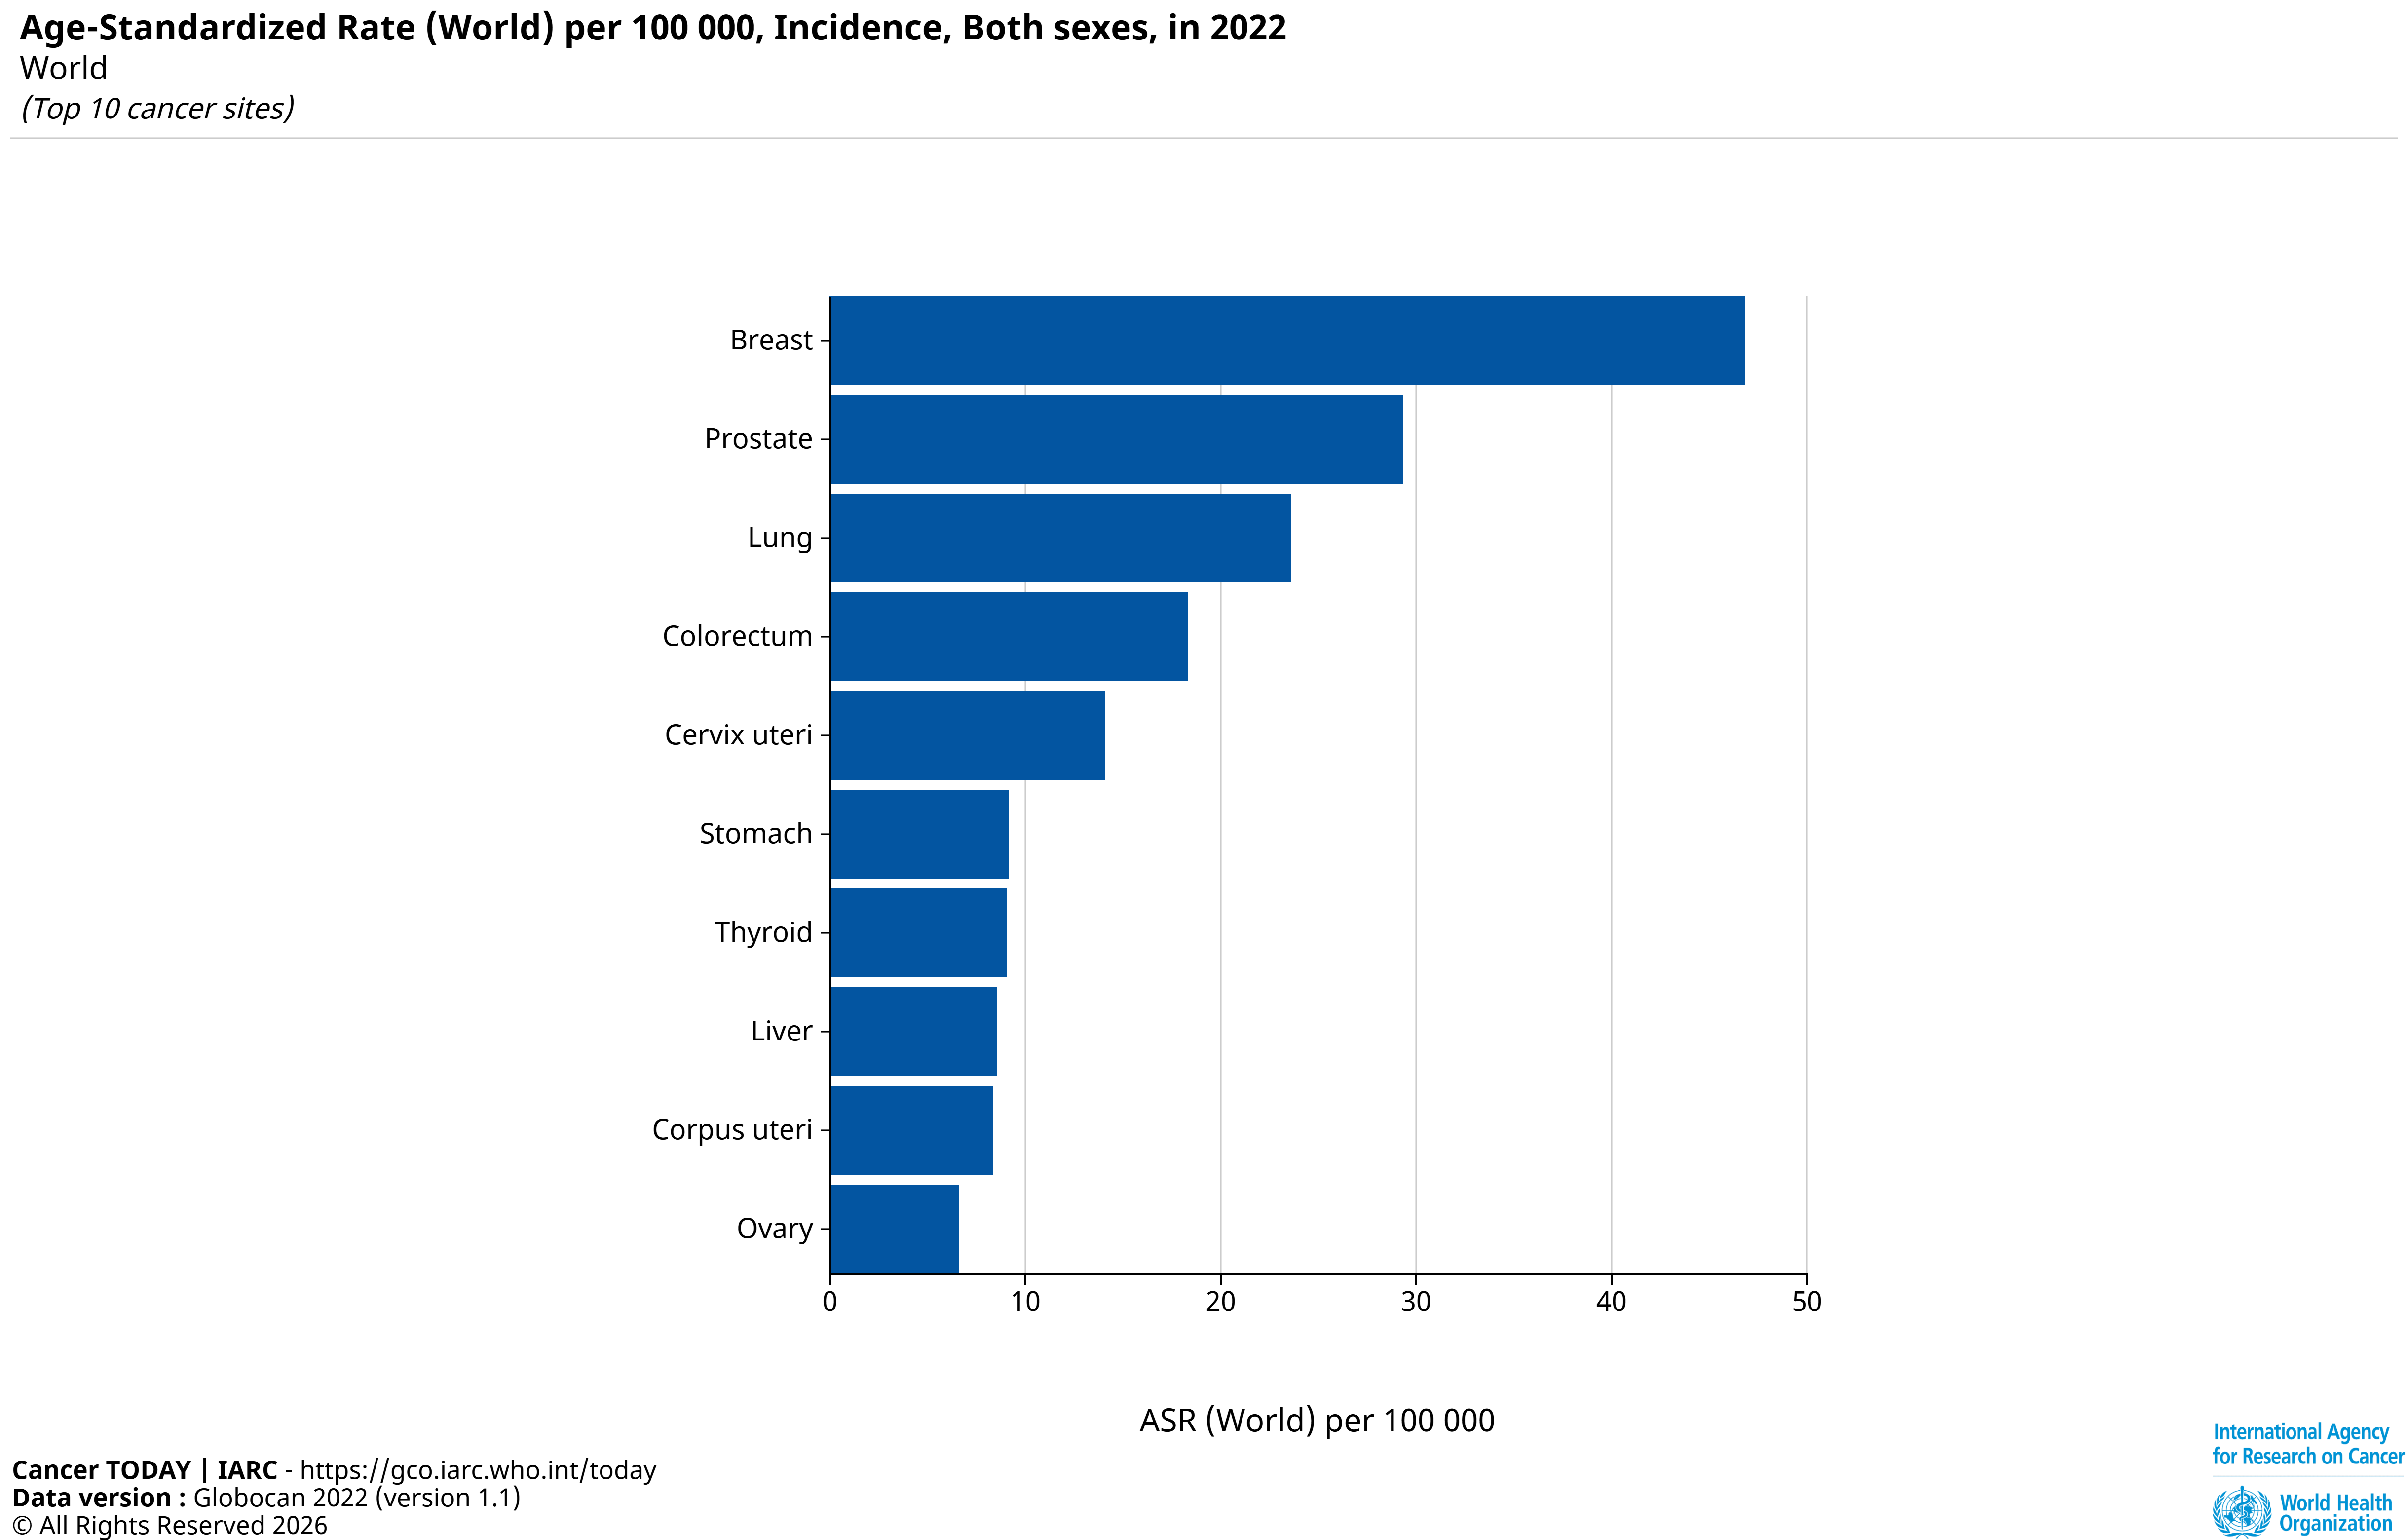
\includegraphics[width=0.85\textwidth]{img/graphic-asr-inc-both-sexes-in-2022-world.png}
  \caption{Tasa de incidencia estandarizada por edad (ASR, mundo) para los 10
           tipos de cáncer más frecuentes a nivel global en 2022. El
           cáncer de mama ocupa la primera posición. Fuente: Cancer
           TODAY, IARC/WHO.}
  \label{fig:globocan_incidencia}
\end{figure}

Esto lo convierte en un caso de uso idóneo para este trabajo: existe una cohorte pública bien documentada (TCGA-BRCA, con más de 1.000 muestras tumorales), los datos están disponibles libremente y el problema de integrar distintas fuentes es representativo del tipo de trabajo habitual en bioinformática.

\section{Repositorios públicos de datos}

\subsection{Gene Expression Omnibus (GEO)}

Gene Expression Omnibus (GEO) es un repositorio público del NCBI que almacena datos de expresión génica y epigenómica generados por la comunidad científica internacional \cite{clough_ncbi_2023}. Recoge experimentos de microarray, RNA-seq y otras tecnologías de alto rendimiento, con sus datos procesados y metadatos. Internamente organiza la información en tres niveles:

\begin{itemize}
\item Plataformas (GPL)
\item Series (GSE)
\item Muestras (GSM)
\end{itemize}

Cada serie agrupa las muestras de un mismo experimento y sus características se guardan como campos que varían entre estudios.

El acceso programático se realiza a través de las E-utilities del NCBI o de librerías especializadas, como GEOparse en Python \cite{gumienny_geoparse_nodate} o GEOquery en R \cite{davis_geoquery_2007}.

\subsection{The Cancer Genome Atlas (TCGA)}

The Cancer Genome Atlas (TCGA) es una iniciativa del National Cancer Institute (NCI) que ha generado perfiles moleculares de una amplia colección de tumores humanos, incluyendo el cáncer de mama \cite{national_cancer_institute_nci_using_nodate}.

El acceso se realiza a través del Genomic Data Commons (GDC) Data Portal \cite{noauthor_gdc_nodate}, que expone una API REST pública para la consulta y descarga de ficheros y sirve de base al paquete TCGAbiolinks de R \cite{colaprico_tcgabiolinks_2015}.

\section{El problema de la heterogeneidad entre fuentes}

GEO y TCGA no organizan la información exactamente igual. Aunque ambos contienen datos de expresión génica, cada fuente usa su propio formato y su propia forma de nombrar los genes.

Por eso, antes de comparar o combinar datos, hace falta un paso de mapeo que traduzca todos los identificadores a un vocabulario común. En este trabajo se usa Ensembl como identificador interno y HGNC como referencia para resolver ambigüedades y mantener los nombres de gen de forma coherente entre fuentes \cite{seal_genenamesorg_2022}.

\section{Herramientas y frameworks existentes}

Durante el máster se han visto varias herramientas orientadas a trabajar con este tipo de datos. La mayoría están en R, dentro del ecosistema Bioconductor: \textit{GEOquery} \cite{davis_geoquery_2007} para descargar datos de GEO, \textit{TCGAbiolinks} \cite{colaprico_tcgabiolinks_2015} para acceder a TCGA vía la API del GDC, y paquetes como \textit{DESeq2} \cite{love_moderated_2014} o \textit{edgeR} \cite{robinson_edger_2009} para la normalización y el análisis de expresión diferencial. La tabla~\ref{tab:herramientas} resume estas herramientas.

\begin{table}[htbp]
\caption{Herramientas principales para el acceso y análisis de datos de expresión génica en repositorios públicos.}
\label{tab:herramientas}
\centering
\begin{tabular}{llll}
\toprule
\textbf{Herramienta} & \textbf{Lenguaje} & \textbf{Fuente} & \textbf{Función principal} \\
\midrule
GEOquery     & R & GEO        & Descarga y parseo de series \\
TCGAbiolinks & R & TCGA (GDC) & Consulta, descarga y análisis \\
DESeq2       & R & --         & Normalización y expresión diferencial \\
edgeR        & R & --         & Expresión diferencial \\
GEOparse     & Python & GEO  & Descarga y parseo de series \\
PyDESeq2     & Python & --   & Reimplementación de DESeq2 \\
\midrule
\end{tabular}
\end{table}

En Python la oferta de librerías es más limitada. GEOparse \cite{gumienny_geoparse_nodate} permite descargar y parsear datos de GEO desde la API del NCBI de forma cómoda, pero no cubre TCGA ni incluye funcionalidades de normalización. Para TCGA existe la opción de usar directamente la API REST del GDC, que es lo que se ha hecho en este trabajo. PyDESeq2 es una reimplementación en Python del método DESeq2, aunque todavía no se ha explorado en detalle.

\section{Limitaciones que motivan este trabajo}

Estas herramientas están fragmentadas: cada una cubre una fuente o una tarea concreta y combinarlas en un flujo de trabajo cohesionado requiere mucho trabajo manual. GEO y TCGA usan formatos y convenciones distintas y no hay nada que lo resuelva de forma integrada en Python.

A eso se suma que muchos análisis que se ven publicados son difíciles de reproducir porque dependen de scripts que habitualmente no están bien documentados. Construir un pipeline modular con esta arquitectura es una forma directa de abordar ese problema.

En este trabajo se usa un entorno empaquetado en contenedores Docker para poder levantar todo el sistema con un solo comando y en cualquier máquina, las dependencias de librerías de python están descritas en el fichero \texttt{requirements.txt}, para el control de versiones se utiliza git y cada paso del procesado se ejecuta mediante comandos documentados.

Estas dos cuestiones, la fragmentación y la reproducibilidad, son el punto de partida de este trabajo.

% ============================================================
% CAPÍTULO 2 OBJETIVOS
% ============================================================

\chapter{Objetivos}

\section{Objetivo general}

El objetivo general de este Trabajo Fin de Máster es explorar la viabilidad de integrar datos de expresión génica de cáncer de mama procedentes de los repositorios públicos GEO y TCGA en un sistema que permita trabajar con ellos de forma coherente y construir sobre esa base un pipeline de análisis reproducible.

\section{Objetivos específicos}

\begin{enumerate}
  \item \textbf{Analizar las herramientas existentes:} revisar qué soluciones hay disponibles para acceder, descargar y procesar datos de GEO y TCGA, evaluando su alcance, limitaciones y posibilidades de uso en este trabajo.
  \item \textbf{Explorar la estructura y disponibilidad de los datos:} examinar qué datos concretos están disponibles en ambos repositorios para el cáncer de mama, qué formatos tienen, qué metadatos clínicos incluyen y qué nivel de homogeneidad existe entre fuentes.
  \item \textbf{Definir una estrategia de integración:} a partir del análisis anterior, decidir cómo unificar los datos de ambas fuentes bajo un modelo común que permita consultarlos y utilizarlos conjuntamente.
  \item \textbf{Diseñar una solución de almacenamiento:} determinar cómo almacenar los datos integrados de forma que sean fácilmente consultables y reutilizables en análisis posteriores.
  \item \textbf{Desarrollar un prototipo funcional:} implementar una primera versión del pipeline que cubra al menos la descarga, integración y almacenamiento de datos de ambas fuentes, como demostración de viabilidad.
  \item \textbf{Evaluar la capacidad predictiva de los datos integrados:} aplicar un clasificador supervisado sobre los datos para comprobar si se puede predecir el subtipo PAM50 y si la predicción se mantiene al cambiar de plataforma.
\end{enumerate}

% ============================================================
% CAPÍTULO 3 MATERIAL Y MÉTODOS
% ============================================================

\chapter{Material y métodos}

\section{Arquitectura del sistema}

El sistema se estructura en dos capas que se despliegan juntas con Docker y Docker Compose.

La containerización de Docker nos permite tener todas las herramientas de desarrollo y ejecución empaquetadas y aisladas del sistema operativo, de modo que el entorno completo se pueda levantar en cualquier máquina con un único comando. La figura~\ref{fig:arquitectura} muestra la arquitectura completa.

La parte de Docker Compose nos permite la orquestación de los servicios necesarios para ejecutar el pipeline, los servicios existentes son:

\begin{itemize}
  \item \textbf{Base de datos PostgreSQL:} almacena los datos descargados y procesados, con un esquema relacional definido mediante el ORM de Django.
  \item \textbf{Aplicación Django:} contiene el modelo de datos, los conectores a las APIs externas, la lógica de procesado y los comandos de gestión que permiten ejecutar cada paso del pipeline.
\end{itemize}

Dentro de la aplicación, el código está repartido en módulos con diferentes roles:

\begin{itemize}
  \item \textbf{Conectores} (\texttt{connectors.py}): acceden a las APIs externas, tanto a las E-utilities del NCBI para GEO como a la API REST del GDC para TCGA, además de la descarga del fichero completo de HGNC.
  \item \textbf{Parsers} (\texttt{parsers.py}): convierten los ficheros descargados (TSV de expresión y MAF de mutaciones) en tablas que se pueden almacenar.
  \item \textbf{Pipeline} (\texttt{pipeline.py}): orquesta la descarga, el parseo y la persistencia de los ficheros, registrando el estado de cada uno.
  \item \textbf{Comandos de gestión}: exponen operaciones del pipeline como una orden de Django (\texttt{python manage.py ...}).
\end{itemize}

La conexión a la base de datos se configura mediante variables de entorno, por lo que se puede apuntar a otra instancia sin modificar el código. La figura~\ref{fig:arquitectura} muestra el esquema completo.

\begin{figure}[htbp]
\centering
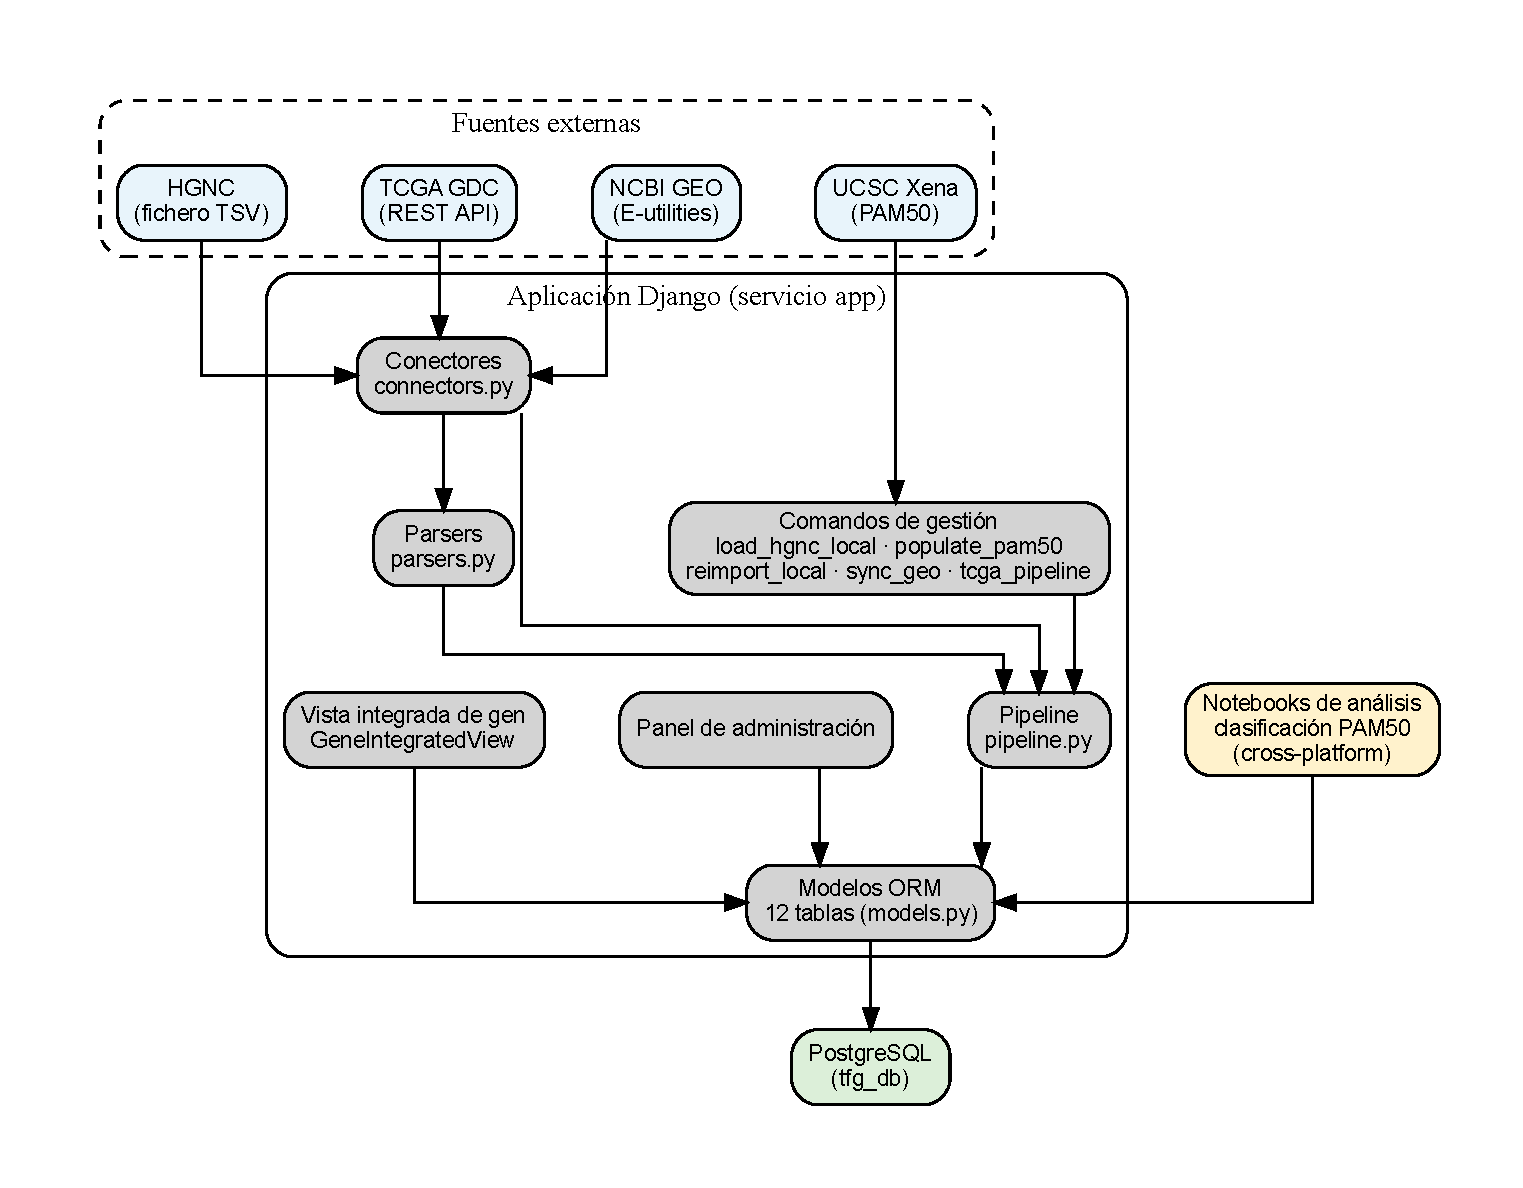
\includegraphics[width=0.95\textwidth]{figures_nuevas/arquitectura.pdf}
\caption[Arquitectura del sistema de integración de datos.]{Arquitectura del sistema: fuentes externas, aplicación Django con sus módulos, base de datos PostgreSQL y notebooks de análisis.}
\label{fig:arquitectura}
\end{figure}

\subsection{Despliegue y reproducción del entorno}

El entorno de desarrollo utiliza Python \cite{noauthor_python_nodate} con conda como gestor de entornos virtuales y las dependencias declaradas en un fichero \texttt{requirements.txt}. El código se gestiona con git.

El despliegue del proyecto se ha realizado con Docker Compose, de forma que el entorno completo puede levantarse en una sola máquina sin necesidad de instalar manualmente PostgreSQL, Django o las dependencias del análisis.

La estructura del repositorio separa claramente la orquestación del sistema (\texttt{src/compose.yml}) de la aplicación (\texttt{src/app/}), de modo que cada componente tiene un objetivo específico y el ciclo de despliegue es reproducible.

La parte de infraestructura se compone de dos servicios principales:
\begin{itemize}
\item \texttt{db}, servicio de base de datos PostgreSQL 15.3
\item \texttt{app}, aplicación Django con las dependencias declaradas en \texttt{requirements.txt}.
\end{itemize}

Durante la fase inicial el contenedor de la aplicación queda configurado para ejecutar la parte web del proyecto y también para servir de punto de entrada a las tareas de ingestión y análisis, de modo que la misma base de código puede usarse tanto para la API y la interfaz como para la preparación de datos.

La reproducción del entorno sigue una secuencia lógica:

\begin{enumerate}
  \item Arrancar los servicios con Docker Compose \texttt{docker compose up -d}.
  \item Aplicar las migraciones de Django para crear el esquema de la base de datos. \texttt{python manage.py migrate}
  \item Cargar la referencia HGNC para resolver los identificadores de genes.  \texttt{python manage.py load\_hgnc\_local}
\end{enumerate}

Finalmente se ejecutan los comandos de población y reimportación de datos. Esta separación por etapas no solo facilita la depuración, sino que también permite volver a reconstruir el estado del sistema desde cero en cualquier entorno con Docker, evitando que el trabajo dependa de una máquina concreta o de pasos manuales ocultos.

El código fuente del proyecto se distribuye bajo un repositorio público de GitHub, disponible en \url{https://github.com/dowdyph0/tfm-bio-unir}, que incluye la aplicación, los conectores, los parsers y los cuadernos de análisis.

\subsection{Flujo operativo del pipeline}

La ejecución del proyecto se puede entender como una secuencia de pasos con estados claros y objetivos bien definidos. La figura~\ref{fig:flujo_pipeline} resume el flujo, separando la rama de GEO (izquierda) de la de TCGA (derecha).

\begin{figure}[htbp]
\centering
\begin{tikzpicture}[node distance=0.6cm]

% rama GEO
\node[draw=unirblue, thick, rounded corners=2pt, fill=white, align=center, text width=4.4cm, font=\small, inner sep=4pt] (g1) {\textbf{1.} Conector GEO\\ \textit{series, muestras, campos clínicos}};
\node[draw=unirblue, thick, rounded corners=2pt, fill=white, align=center, text width=4.4cm, font=\small, inner sep=4pt, below=of g1] (g2) {\textbf{2.} Descarga SOFT + plataforma};
\node[draw=unirblue, thick, rounded corners=2pt, fill=white, align=center, text width=4.4cm, font=\small, inner sep=4pt, below=of g2] (g3) {\textbf{3.} Mapeo de sondas\\ \textit{probe $\rightarrow$ Entrez $\rightarrow$ HGNC}};
\node[draw=unirblue, thick, rounded corners=2pt, fill=white, align=center, text width=4.4cm, font=\small, inner sep=4pt, below=of g3] (g4) {\textbf{4.} Etiquetas PAM50\\ \textit{metadatos de muestras}};
\node[draw=unirblue, thick, rounded corners=2pt, fill=white, align=center, text width=4.4cm, font=\small, inner sep=4pt, below=of g4] (g5) {\textbf{5.} z-score por gen};

% rama TCGA
\node[draw=unirblue, thick, rounded corners=2pt, fill=white, align=center, text width=4.4cm, font=\small, inner sep=4pt, right=2.6cm of g1] (t1) {\textbf{1.} Conector TCGA\\ \textit{proyectos, ficheros, casos}};
\node[draw=unirblue, thick, rounded corners=2pt, fill=white, align=center, text width=4.4cm, font=\small, inner sep=4pt, below=of t1] (t2) {\textbf{2.} Descarga y parseo\\ \textit{TSV + MAF}};
\node[draw=unirblue, thick, rounded corners=2pt, fill=white, align=center, text width=4.4cm, font=\small, inner sep=4pt, below=of t2] (t3) {\textbf{3.} Mapeo Ensembl $\rightarrow$ HGNC};
\node[draw=unirblue, thick, rounded corners=2pt, fill=white, align=center, text width=4.4cm, font=\small, inner sep=4pt, below=of t3] (t4) {\textbf{4.} Etiquetas PAM50\\ \textit{matriz UCSC Xena}};

% cabeceras de rama
\node[font=\small\bfseries, text=unirblue, above=0.35cm of g1] {GEO (GSE25055)};
\node[font=\small\bfseries, text=unirblue, above=0.35cm of t1] {TCGA (TCGA-BRCA)};

% artefactos
\node[draw=unirblue, very thick, rounded corners=2pt, fill=unirbluelight, align=center, text width=5.4cm, font=\small, inner sep=5pt] (art) at ($(g5.south)!0.5!(t4.south) + (0,-2.4cm)$) {\textbf{Artefactos de análisis}\\ \textit{notebooks $\rightarrow$ figuras, tablas, métricas}};

% flechas
\draw[-latex, thick, unirblue] (g1) -- (g2);
\draw[-latex, thick, unirblue] (g2) -- (g3);
\draw[-latex, thick, unirblue] (g3) -- (g4);
\draw[-latex, thick, unirblue] (g4) -- (g5);
\draw[-latex, thick, unirblue] (t1) -- (t2);
\draw[-latex, thick, unirblue] (t2) -- (t3);
\draw[-latex, thick, unirblue] (t3) -- (t4);
\draw[-latex, thick, unirblue] (g5) -- (art);
\draw[-latex, thick, unirblue] (t4) -- (art);
\end{tikzpicture}
\caption[Flujo operativo del pipeline por fuente.]{Flujo operativo del pipeline: rama GEO (izquierda) y rama TCGA (derecha). Ambas convergen en los artefactos de análisis; el mapeo de genes se apoya en la referencia HGNC.}
\label{fig:flujo_pipeline}
\end{figure}

En la rama GEO (izquierda), el paso 1 consulta las series disponibles y devuelve sus muestras y campos clínicos; el paso 2 descarga el fichero SOFT de la serie y su plataforma; el paso 3 traduce cada sonda a su gen mediante Entrez y HGNC; el paso 4 extrae la etiqueta PAM50 de los metadatos de cada muestra; y el paso 5 calcula el z-score por gen y guarda los registros finales.

En la rama TCGA (derecha), el paso 1 consulta los proyectos, ficheros y casos del GDC; el paso 2 descarga y parsea los ficheros (TSV de expresión y MAF de mutaciones); el paso 3 traduce los identificadores Ensembl a HGNC; y el paso 4 asigna la etiqueta PAM50 cruzando cada caso con la matriz clínica de UCSC Xena.

Aunque cada rama parte de identificadores distintos, ambas quedan alineadas por la referencia HGNC, de modo que los genes de GEO y TCGA resultan comparables. En TCGA, cada descarga registra su estado (descargado, parseado o fallido) en la base de datos, lo que permite reanudar el flujo sin repetir pasos ya completados. Ambas ramas convergen en los artefactos de análisis: los notebooks leen los datos ya estandarizados y generan las figuras, tablas y métricas, de modo que cada resultado puede rastrearse hasta la fuente que lo generó.

\subsection{Estructura del repositorio y artefactos generados}

El repositorio se organiza como se muestra a continuación; se omiten los directorios auxiliares (cachés, migraciones de Django y ficheros intermedios de compilación):

\begin{minted}[linenos=false]{bash}
tfm-bio-unir/
|-- src/                            # orquestación y aplicación
|   |-- compose.yml                 # servicios db (PostgreSQL) y app (Django)
|   |-- staticfiles/                # estáticos servidos por Django
|   `-- app/
|       |-- Dockerfile              # imagen del contenedor de la aplicación
|       |-- manage.py               # punto de entrada de Django
|       |-- requirements.txt        # dependencias de Python
|       |-- project/                # configuración del proyecto Django
|       `-- core/                   # lógica de negocio
|           |-- connectors.py       # acceso a GEO, TCGA y HGNC
|           |-- parsers.py          # parseo de TSV (expresión) y MAF (mutaciones)
|           |-- pipeline.py         # orquestación y persistencia
|           |-- models.py           # esquema relacional (ORM)
|           |-- views.py            # vistas de la aplicación web
|           `-- management/commands/  # comandos del pipeline
|-- data/                           # referencia HGNC y ejemplos de la API de GEO
|-- downloads/                      # ficheros crudos descargados (TSV y MAF)
|-- notebooks/                      # cuadernos de clasificación PAM50
|-- scripts/                        # utilidades sueltas (prueba sintética)
|-- tex/                            # memoria, figuras y bibliografía
|   |-- figures/                    # figuras generadas por los notebooks
|   `-- img/                        # capturas y esquemas
`-- readme.md                       # descripción general del proyecto
\end{minted}

La separación es deliberada: \texttt{src/} agrupa todo el código que se despliega con Docker, \texttt{data/} y \texttt{downloads/} guardan los datos de referencia y los ficheros descargados, y \texttt{notebooks/} junto con \texttt{tex/} contienen el análisis y la memoria. Los artefactos finales —figuras, tablas y métricas— se generan desde los notebooks y se guardan en \texttt{tex/figures} para incluirlos en el documento.

\subsection{Validación, trazabilidad y control de calidad}

La validación se apoya en dos mecanismos concretos. Por un lado, cada descarga de TCGA registra su estado mediante \texttt{DownloadStatus} (pendiente, descargando, descargado, parseado o fallido), de modo que desde el panel de administración se puede comprobar qué ficheros han quedado procesados y cuáles no. Por otro lado, la reimportación desde disco (\texttt{reimport\_local}) permite reconstruir la base de datos sin volver a contactar con el GDC, lo que facilita repetir el análisis o recuperar el estado tras un fallo.

\section{Conectores de acceso a los repositorios}

Como primer paso práctico se ha desarrollado un módulo de conectores (\texttt{connectors.py}) que conecta con los repositorios y permite comprobar qué datos están disponibles. El módulo implementa tres clases:

\textbf{GEOConnector} utiliza las E-utilities del NCBI: \texttt{esearch} para buscar series por término (por ejemplo, \textit{breast cancer}) y \texttt{esummary} para obtener el resumen de cada una, devolviendo el identificador, el número de muestras y la fecha. También descarga los metadatos completos de una serie concreta mediante GEOparse, incluyendo la tabla de muestras con sus características clínicas.

\textbf{TCGAConnector} utiliza la API REST del GDC: \texttt{/projects} para listar proyectos, \texttt{/files} para consultar ficheros aplicando filtros (por ejemplo, la expresión génica de TCGA-BRCA), \texttt{/cases} para los metadatos clínicos y \texttt{/data/\{file\_id\}} para descargar un fichero concreto.

\textbf{HGNCConnector} descarga el fichero completo de HGNC desde el almacenamiento público para construir la tabla de referencia que permite traducir identificadores de genes entre fuentes.

Las figuras \ref{fig:conector1} a \ref{fig:conector4} muestran la salida obtenida al ejecutar el script contra ambas APIs, formateada en consola con la librería Rich \cite{noauthor_rich_nodate}. Los resultados muestran la diferencia entre fuentes: GEO ofrece series con distintas plataformas (microarray, NanoString, RNA-seq) y tamaños muy variables, mientras que TCGA-BRCA presenta ficheros de expresión en formato RNA-seq estandarizado.

\begin{figure}[htbp]
\centering
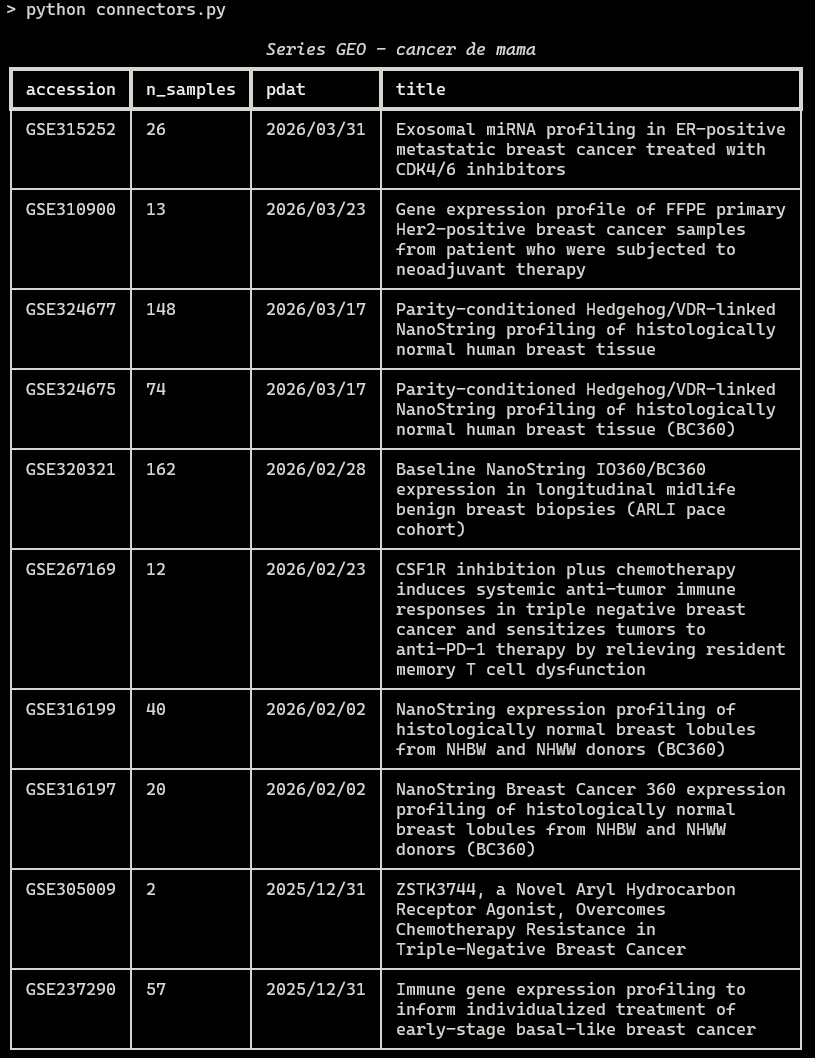
\includegraphics[width=0.9\textwidth]{img/conector1.png}
\caption[Series GEO de cáncer de mama (GEOConnector).]{Series GEO de cáncer de mama obtenidas mediante \texttt{GEOConnector.search()}.}
\label{fig:conector1}
\end{figure}

\begin{figure}[htbp]
\centering
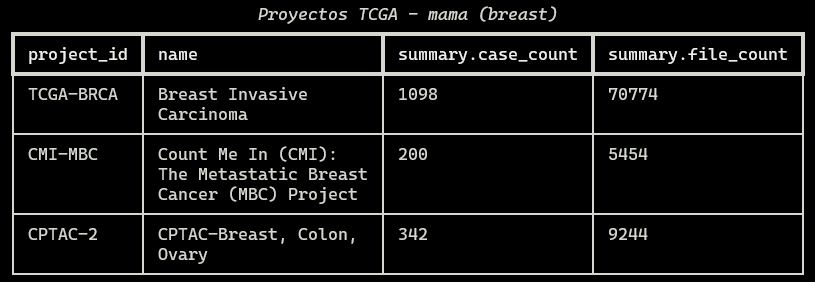
\includegraphics[width=0.9\textwidth]{img/conector2.png}
\caption[Proyectos TCGA de cáncer de mama (TCGAConnector).]{Proyectos TCGA relacionados con cáncer de mama obtenidos mediante \texttt{TCGAConnector.list\_projects()}.}
\label{fig:conector2}
\end{figure}

\begin{figure}[htbp]
\centering
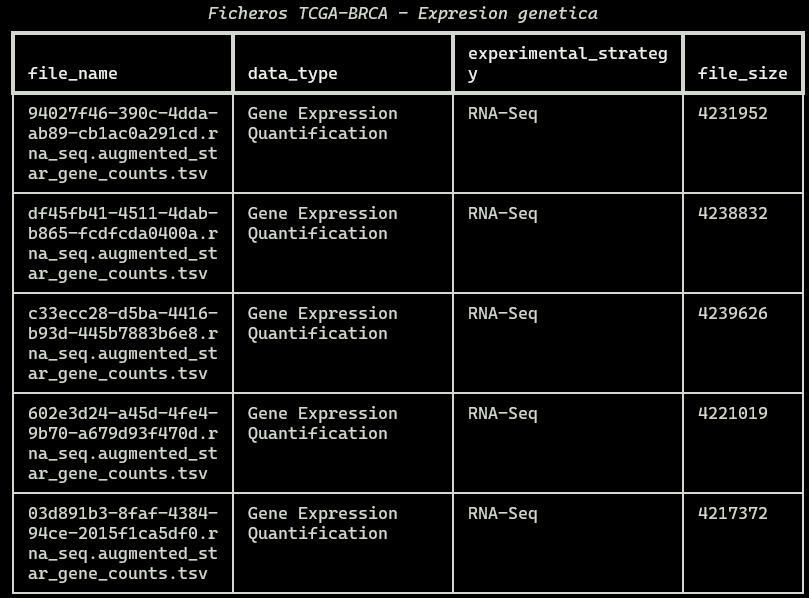
\includegraphics[width=0.9\textwidth]{img/conector3.png}
\caption[Ficheros de expresión génica de TCGA-BRCA (TCGAConnector).]{Primeros ficheros de expresión génica de TCGA-BRCA obtenidos mediante \texttt{TCGAConnector.list\_files()}.}
\label{fig:conector3}
\end{figure}

\begin{figure}[htbp]
\centering
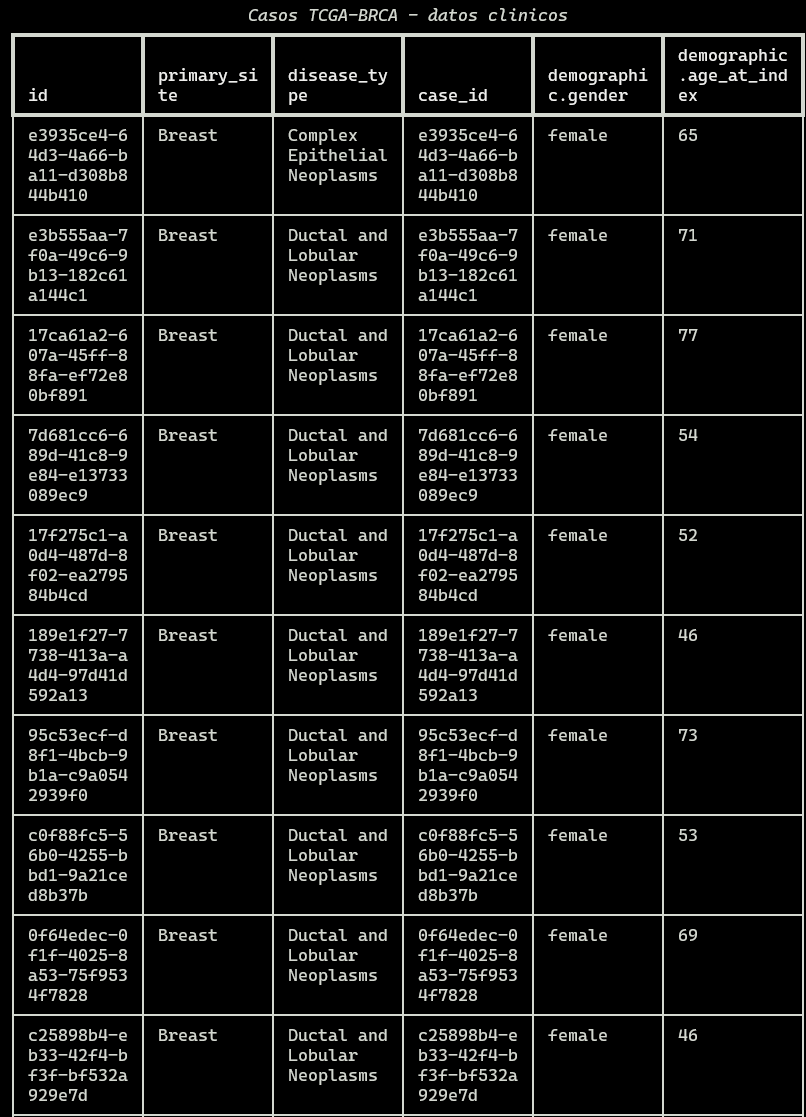
\includegraphics[width=0.9\textwidth]{img/conector4.png}
\caption[Metadatos clínicos de TCGA-BRCA (TCGAConnector).]{Muestra de metadatos clínicos de TCGA-BRCA obtenidos mediante \texttt{TCGAConnector.get\_clinical\_summary()}.}
\label{fig:conector4}
\end{figure}

\section{Modelo de datos}

Para el almacenamiento y gestión de los datos descargados se ha optado por una base de datos relacional gestionada mediante el ORM de Django, un framework web de Python que permite definir el esquema de datos en código y manejar la base de datos sin escribir secuencias SQL, ya que los datos de TCGA y GEO tienen una estructura estable que se puede reflejar en un esquema fijo.

El esquema se organiza en cuatro bloques (figura~\ref{fig:erd}): TCGA, GEO, la referencia de genes HGNC y los resultados del módulo de aprendizaje.

El bloque de tablas TCGA contiene:

\begin{itemize}
  \item \texttt{TCGAProject}: almacena los proyectos del GDC, como TCGA-BRCA.
  \item \texttt{TCGACase}: almacena los casos clínicos, con su subtipo molecular.
  \item \texttt{TCGAFile}: almacena los ficheros, enlazados a sus casos mediante una relación muchos a muchos.
  \item \texttt{DownloadStatus}: registra el estado de cada descarga a lo largo del pipeline (\textit{pending}, \textit{downloading}, \textit{downloaded}, \textit{parsed} o \textit{failed}).
  \item \texttt{TCGAExpressionRecord}: almacena los registros de expresión de cada fichero, con las columnas del formato STAR (conteos y TPM).
  \item \texttt{TCGAMutation}: almacena las mutaciones detectadas en cada caso.
\end{itemize}

El bloque de tablas GEO contiene:

\begin{itemize}
  \item \texttt{GEOSeries}: almacena una entrada por serie.
  \item \texttt{GEOSample}: almacena las muestras, con sus características clínicas en un campo JSON porque varían entre estudios.
  \item \texttt{GEOExpressionRecord}: almacena el valor de expresión y el z-score de cada gen en cada muestra.
\end{itemize}

La tabla \texttt{HGNCGene} actúa de referencia para traducir identificadores de genes entre fuentes (Entrez para GEO, Ensembl para TCGA). 

Por último las tablas \texttt{MLModelRun} y \texttt{MLGeneImportance} guardan los resultados de cada ejecución del clasificador y la importancia de cada gen.

\begin{figure}[htbp]
\centering
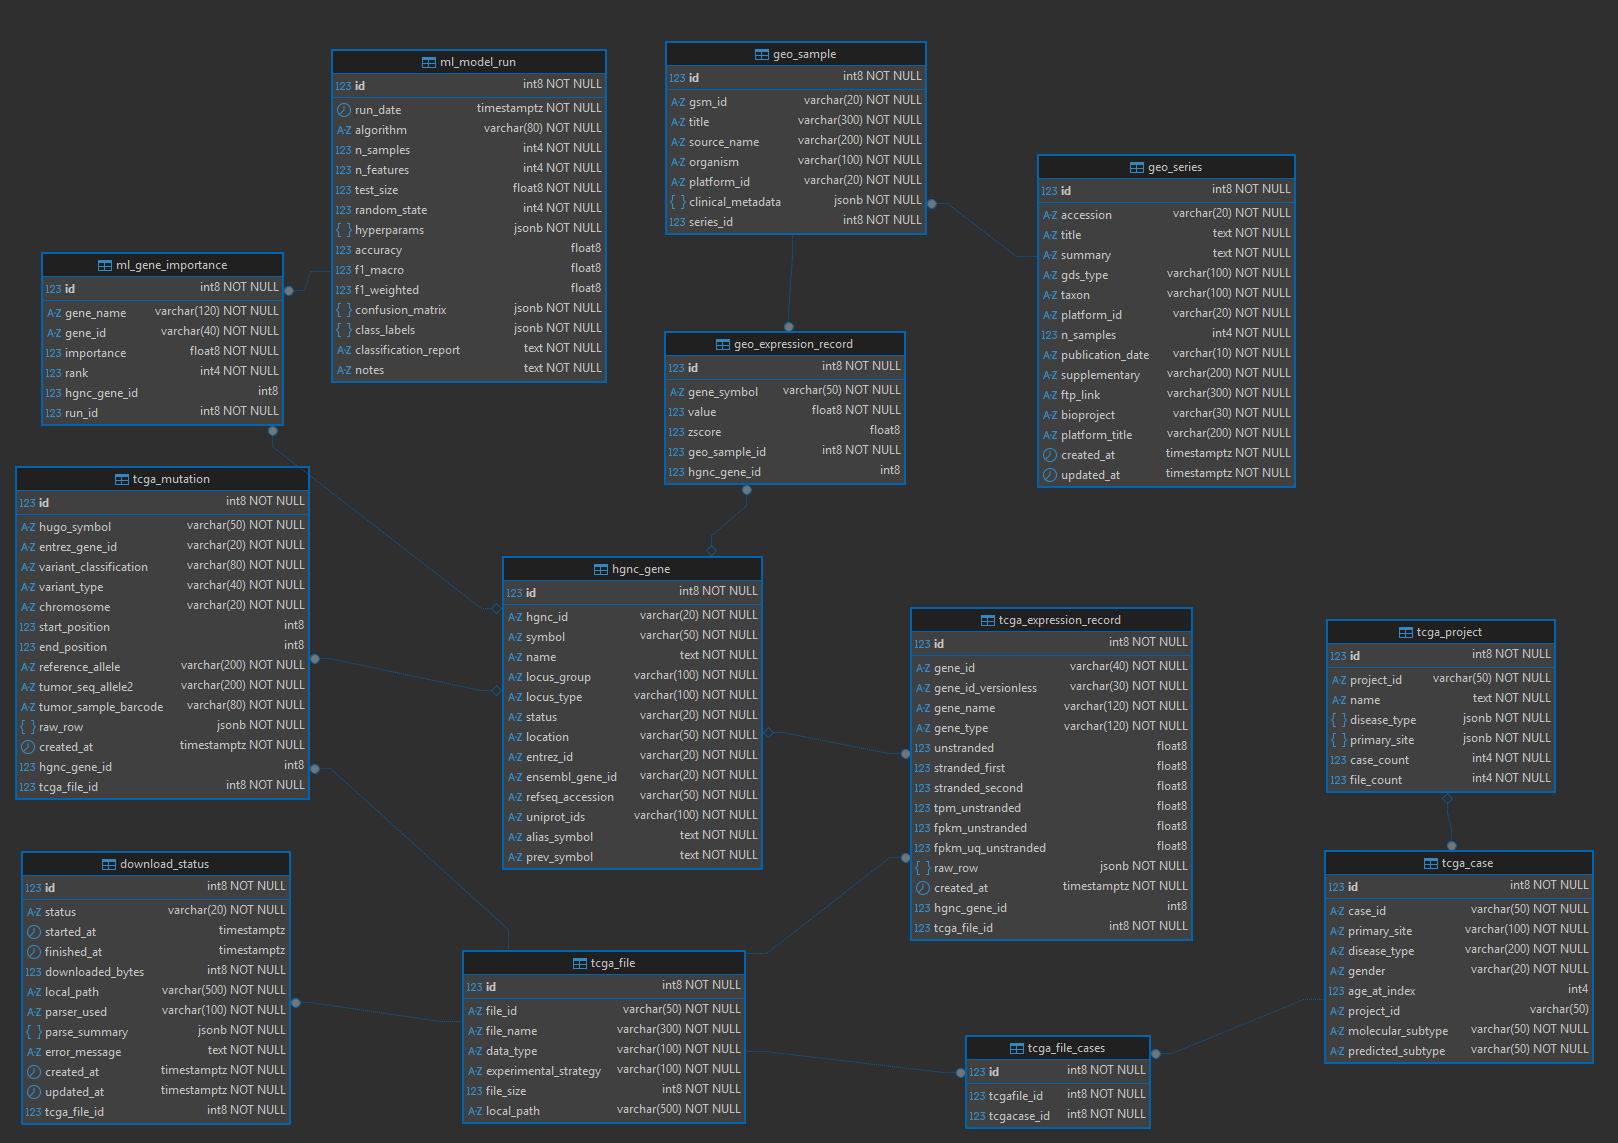
\includegraphics[width=0.9\textwidth]{img/er.png}
\caption[Diagrama entidad-relación del modelo de datos.]{Diagrama entidad-relación generado con DBeaver}
\label{fig:erd}
\end{figure}

\section{Pipeline de procesado e ingestión de datos}

La ingestión de datos se realiza mediante comandos de gestión de Django, cada uno responsable de una etapa del flujo:

\begin{itemize}
  \item \texttt{load\_hgnc\_local} carga la tabla de referencia HGNC desde un fichero local.
  \item \texttt{populate\_pam50} asigna el subtipo PAM50 a los casos de TCGA-BRCA: resuelve el identificador interno de cada caso a su código de muestra y lo cruza con la matriz clínica de UCSC Xena (columna \texttt{PAM50Call\_RNAseq}).
  \item \texttt{tcga\_pipeline} descarga y parsea ficheros de TCGA, registrando el estado de cada fichero.
  \item \texttt{reimport\_local} reconstruye la base de datos desde los ficheros TSV ya descargados en disco, sin volver a contactar con el GDC.
  \item \texttt{sync\_geo} procesa una serie GEO completa: descarga el fichero SOFT y su plataforma, mapea cada sonda a su gen mediante Entrez y HGNC, extrae las etiquetas PAM50 de las muestras, calcula el z-score por gen y almacena los registros.
\end{itemize}

El flujo de \texttt{sync\_geo} ilustra el proceso de integración de identificadores: la plataforma (GPL) indica, mediante el identificador Entrez, qué gen corresponde a cada sonda; ese identificador se traduce al símbolo HGNC consultando la tabla de referencia, de modo que los valores de GEO quedan expresados en el mismo vocabulario que los de TCGA.

\section{Selección de PAM50 como sistema de clasificación}

Se eligió PAM50 porque TCGA-BRCA incluye la etiqueta de subtipo en sus metadatos clínicos, lo que proporciona una etiqueta para poder aplicar entrenamiento supervisado sin necesidad de anotación manual.

Conviene aclarar que en este trabajo no se usan los 50 genes originales de PAM50 como variables de entrada, sino que se deja que el modelo seleccione los genes más importantes de los disponibles.

\section{Diferencias entre plataformas y necesidad de normalización}
En el caso de GEO, el conjunto elegido es el GSE25055 \cite{hatzis_genomic_2011}, un estudio de pacientes con cáncer de mama, cuyas muestras fueron analizadas con microarray y anotadas con subtipo PAM50. Al inspeccionar los datos descargados se observó que GEO GSE25055 contiene datos de microarray en escala logarítmica (log$_2$), mientras que TCGA-BRCA proporciona datos de RNA-seq en unidades TPM (\textit{Transcripts Per Million}).

Son dos tecnologías distintas que miden la expresión con escalas y distribuciones diferentes, por lo que comparar directamente los valores de una fuente con los de la otra no tiene sentido.

Para poder usar un mismo modelo entrenado en TCGA y aplicarlo sobre GEO, hace falta transformar ambas fuentes a una escala común.

\section{Estrategia de normalización y selección de genes}

Los datos vienen de dos fuentes: TCGA-BRCA (RNA-seq, en TPM) y GEO GSE25055 (microarray, en escala log$_2$). Como no comparten unidades, cada una se preparó por separado y al final se dejaron comparables.

\textbf{TCGA-BRCA.} Primero se seleccionaron solo los genes \textit{protein\_coding} (19938). Después se aplicó un logaritmo a los TPM, $x' = \log(1 + x)$, porque cubren un rango enorme y, sin él, los genes con números grandes dominarían al resto (el $+1$ evita el problema de los ceros). Por último se calculó la varianza de cada gen y se seleccionaron los 3000 que más variaban entre muestras, descartando los que se expresan igual en todas.

\textbf{GEO GSE25055.} Aquí no hizo falta el logaritmo, porque sus datos ya vienen en escala log$_2$. Solo se usaron los mismos 3000 genes elegidos en TCGA.

Después, a cada gen de ambas fuentes se le aplicó un z-score:
\[
z_{ij} = \frac{x'_{ij} - \mu_j}{\sigma_j}
\]
donde $x'_{ij}$ es el valor transformado del gen $j$ en la muestra $i$, y $\mu_j$ y $\sigma_j$ son la media y la desviación típica de ese gen. Así cada gen queda con media 0 y varianza 1, y el modelo se fija en cuánto se desvía cada gen respecto a la media de ese gen dentro de su cohorte.

La selección de los 3000 genes se hizo solo con TCGA y antes del z-score. Si se estandariza primero, todos los genes quedan con varianza 1 y ya no se pueden elegir entre ellos. Por último no se tocó GEO en la selección, para que el conjunto de test externo quede completamente aparte.

\section{Modelo de clasificación}

Se eligió Random Forest porque maneja bien un número alto de variables (3000 genes) frente a un número reducido de muestras (221) y captura relaciones no lineales entre genes \cite{breiman_random_2001}. El modelo se configuró con 300 árboles (\texttt{n\_estimators=300}), con balanceo interno de clases (\texttt{class\_weight="balanced"}) y la semilla aleatoria se fijó a 42 para que los resultados sean reproducibles.

\section{Estrategia de validación}

Para medir si el modelo funciona se usaron dos tipos de prueba:

La primera es una validación interna. Se separaron los datos de TCGA en un 80\% para entrenar y un 20\% para probar, de forma estratificada, de modo que cada subtipo conserva su proporción en los dos grupos. Un ejemplo de este reparto se puede ver en la tabla~\ref{tab:split}. El modelo se entrena con el 80\% y se evalúa con el 20\%, que no ha visto. Para que el resultado no dependa de un reparto concreto, se hizo además una validación cruzada de 5 pliegues: se parten los datos en cinco trozos y se entrena cinco veces, cada vez dejando un trozo distinto fuera para probar, y se promedian los resultados.

\begin{table}[htbp]
\caption{Reparto estratificado 80/20 de las 221 muestras TCGA-BRCA por subtipo PAM50.}
\label{tab:split}
\centering
\begin{tabular}{lrrr}
\toprule
\textbf{Subtipo} & \textbf{Total} & \textbf{Entrenamiento (80\%)} & \textbf{Test (20\%)} \\
\midrule
LumA   & 106 & 84 & 22 \\
LumB   &  39 & 31 &  8 \\
Basal  &  31 & 25 &  6 \\
Normal &  30 & 24 &  6 \\
Her2   &  15 & 12 &  3 \\
\midrule
\textbf{Total} & \textbf{221} & \textbf{176} & \textbf{45} \\
\bottomrule
\end{tabular}
\end{table}

La segunda es una validación externa: se entrena con todos los datos de TCGA y se prueba con datos de GEO (microarray en vez de RNA-seq).

Para interpretar los resultados se usan las métricas estándar en clasificación. En este contexto, una \textbf{clase} es cada uno de los cinco subtipos PAM50 que el modelo debe predecir (Luminal A, Luminal B, HER2-enriquecido, Basal y Normal).

\begin{itemize}
  \item \textbf{Accuracy} (exactitud): porcentaje de muestras correctamente clasificadas sobre el total.
  \item \textbf{Precision} (precisión): de todas las muestras que el modelo asigna a un subtipo, cuántas acierta. Una precisión baja en un subtipo significa que el modelo lo confunde con otros.
  \item \textbf{Recall} (exhaustividad): de todas las muestras que realmente son de un subtipo, cuántas encuentra el modelo. Un recall bajo significa que el modelo no detecta ese subtipo.
  \item \textbf{F1}: media armónica de precisión y exhaustividad. Útil cuando las clases están desbalanceadas, porque penaliza que una de las dos sea baja. El F1 macro promedia el F1 de los 5 subtipos tratándolos por igual, sin importar cuántas muestras tenga cada uno. El F1 weighted, en cambio, pondera cada subtipo por su número de muestras.
  \item \textbf{Macro avg} (media macro): promedio simple de la métrica en los 5 subtipos, tratándolos por igual.
  \item \textbf{Weighted avg} (media ponderada): promedio de la métrica ponderado por el número de muestras de cada subtipo.
  \item \textbf{Support} (soporte): número de muestras reales de cada subtipo en el conjunto evaluado.
  \item \textbf{AUC-ROC}: área bajo la curva ROC, que mide lo bien que el modelo separa cada subtipo del resto. Como hay cinco subtipos, se calcula un AUC por cada uno (cada clase contra las demás) y se promedian para obtener el AUC macro. Es menos sensible al desbalance de clases que la exactitud\footnote{La curva ROC (\textit{Receiver Operating Characteristic}) dibuja, para cada nivel de exigencia, cuántos aciertos logra el modelo frente a cuántos errores comete. Un AUC de 1,0 es una separación perfecta y 0,5 equivale a decidir al azar.}.
\end{itemize}

Todas estas métricas, salvo el soporte, toman valores entre 0 y 1 (o entre 0\% y 100\% si se expresan en porcentaje): 1 es el mejor resultado posible y 0, el peor. Por ejemplo, una precisión de 1 significa que todas las muestras asignadas a un subtipo eran correctas, y una precisión de 0 significa que ninguna lo era.

La precisión y la exhaustividad se calculan por clase a partir de los verdaderos positivos ($VP_k$), falsos positivos ($FP_k$) y falsos negativos ($FN_k$) de cada clase $k$:
\[
\text{Precisión}_k = \frac{VP_k}{VP_k + FP_k}, \qquad \text{Recall}_k = \frac{VP_k}{VP_k + FN_k}.
\]
El F1 de cada clase es la media armónica de ambas, y la exactitud global es la proporción de muestras correctamente clasificadas sobre el total:
\[
F1_k = 2 \cdot \frac{\text{Precisión}_k \cdot \text{Recall}_k}{\text{Precisión}_k + \text{Recall}_k}, \qquad
\text{Accuracy} = \frac{\text{aciertos}}{\text{total}}.
\]

\section{Validación del método con datos sintéticos}

Para comprobar que el pipeline descrito es correcto con independencia de los datos reales, se realizó una prueba con datos sintéticos generados a partir de señal conocida. Se simula una cohorte con la misma estructura que la real (221 muestras y cinco subtipos PAM50) y 19\,938 genes, de los cuales un subconjunto de marcadores porta una señal de clase específica de cada subtipo mientras que el resto es ruido. Sobre esa matriz se aplica exactamente el mismo procesado que en la memoria (log1p, selección de los 3000 genes de mayor varianza, z-score por gen) y el mismo clasificador Random Forest. El fragmento siguiente recoge la parte esencial del script:

\inputminted[firstline=27,lastline=78]{python}{../scripts/prueba_sintetica.py}

El resultado de esta prueba es concluyente: el modelo recupera la señal sintética con una exactitud y un F1 macro de 1,0 en la partición de test y un F1 macro de 1,0 $\pm$ 0,0 en la validación cruzada, frente a un nivel de azar de aproximadamente 0,20 para cinco clases. Que el clasificador acierte la totalidad de las muestras cuando la señal es conocida confirma que el procesado y el algoritmo son capaces de aprender subtipos a partir de la expresión génica normalizada. Por otro lado, podemos ver que el rendimiento sobre los datos reales es más bajo y esto es una consecuencia de la dificultad del problema.

% ============================================================
% CAPÍTULO 4 RESULTADOS
% ============================================================

\chapter{Resultados}

\section{Infraestructura de datos y almacenamiento}

La base de datos PostgreSQL cuenta con 1098 casos clínicos de TCGA-BRCA, de los cuales 843 disponen de etiqueta de subtipo PAM50. La tabla de referencia génica contiene 44982 entradas HGNC. Se han ingestado 17,7 millones de registros de expresión génica procedentes de 292 ficheros RNA-seq en formato TSV (\texttt{augmented\_star\_gene\_counts}), que cubren 60664 genes por muestra. Las figuras~\ref{fig:admin1} y \ref{fig:admin2} muestran los registros accesibles desde el panel de administración de Django.

La tabla~\ref{tab:bd_resumen} resume el contenido de la base de datos tras completar la ingestión.

\begin{table}[htbp]
\caption{Resumen del contenido de la base de datos al finalizar la ingestión.}
\label{tab:bd_resumen}
\centering
\begin{tabular}{lrr}
\toprule
\textbf{Elemento} & \textbf{Registros} \\
\midrule
Casos clínicos TCGA-BRCA & 1098 \\
Casos con subtipo PAM50 & 843 \\
Ficheros RNA-seq descargados & 292 \\
Registros de expresión génica (TCGA) & 17713888 \\
Genes en la referencia HGNC & 44982 \\
Muestras GEO GSE25055 & 310 \\
Registros de expresión GEO & 3979160 \\
\midrule
\end{tabular}
\end{table}

\begin{figure}[htbp]
\centering
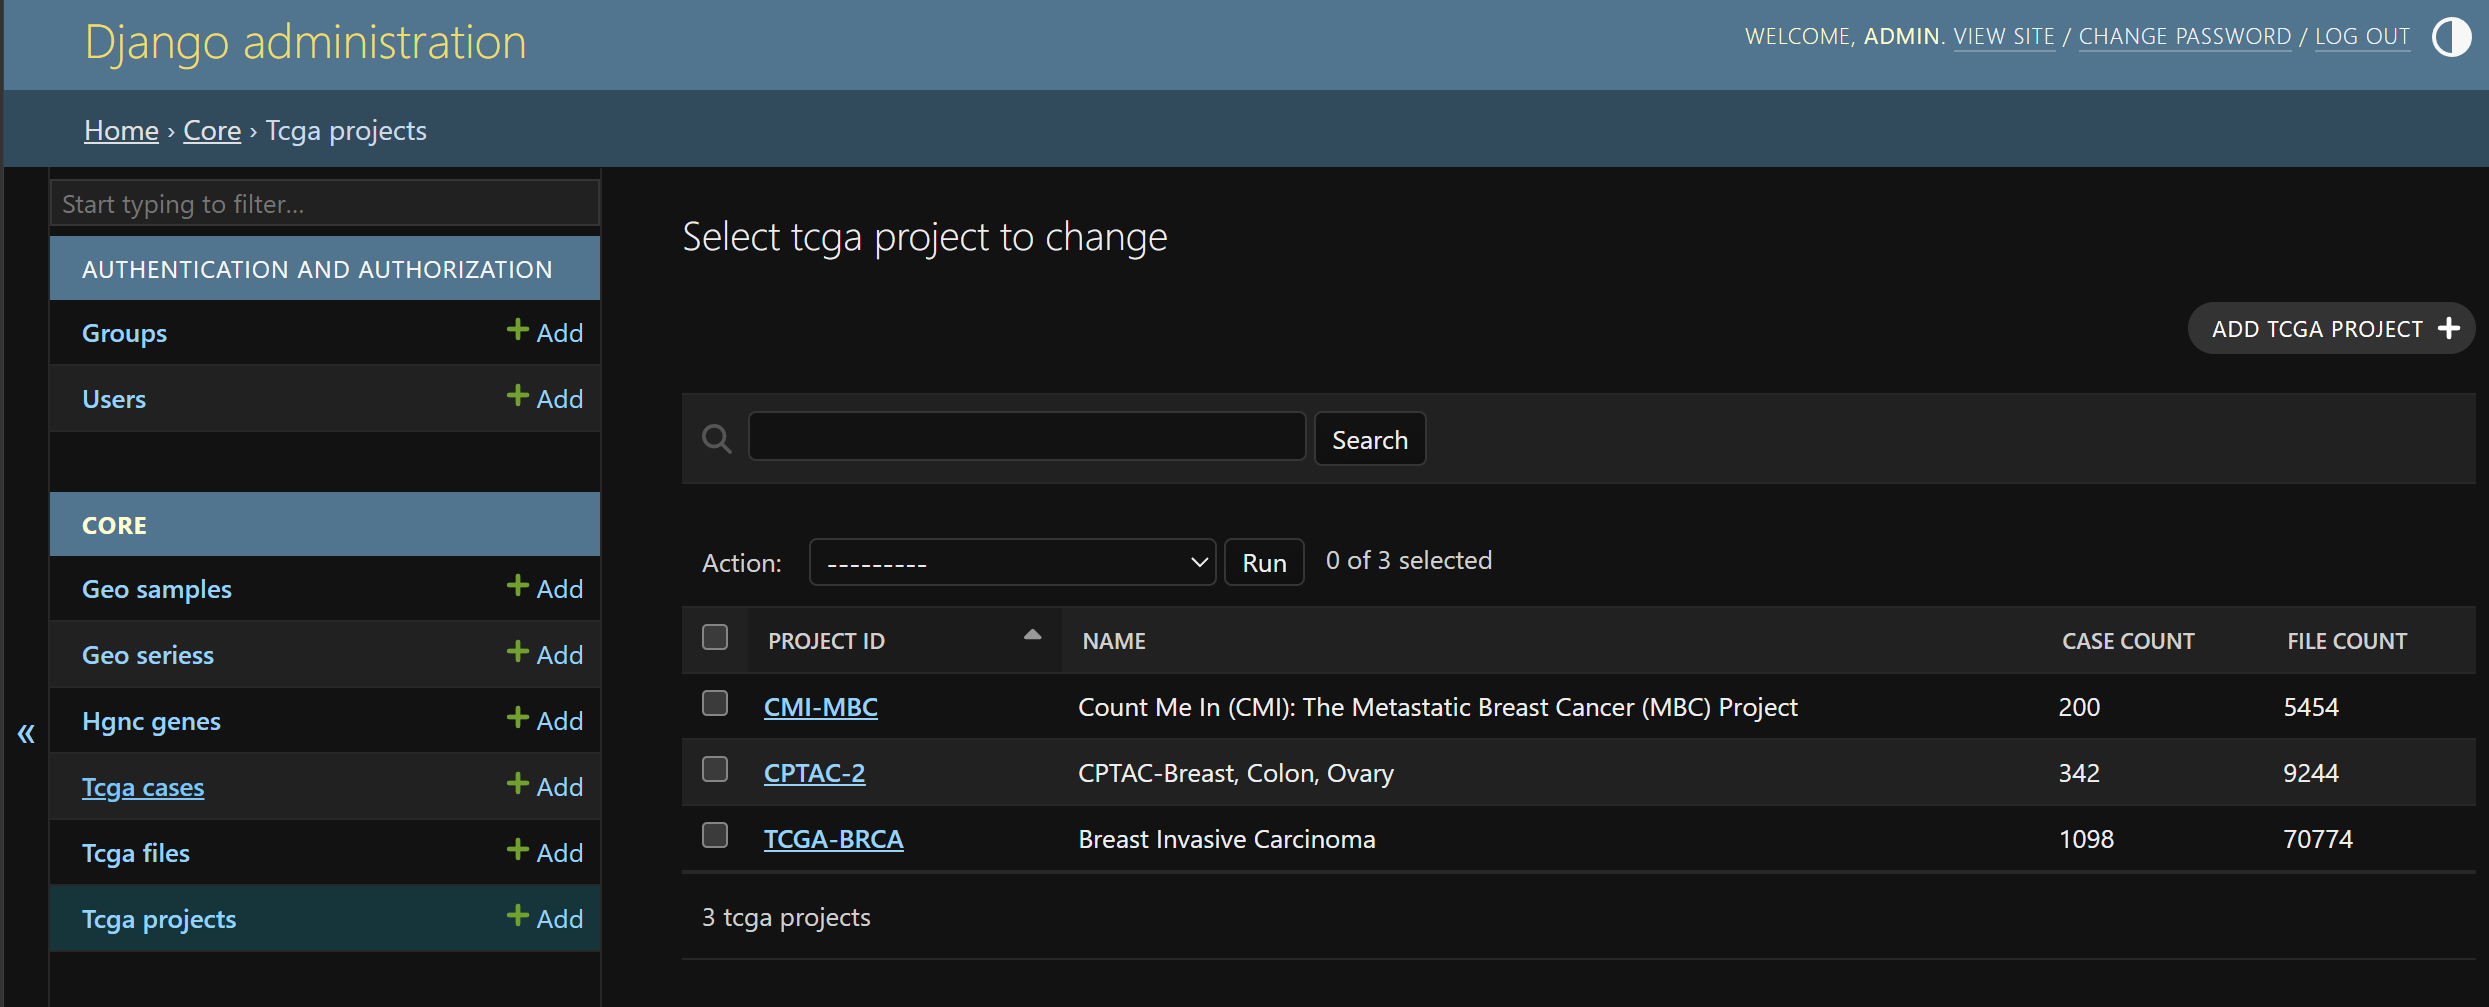
\includegraphics[width=0.9\textwidth]{img/django-admin-tcgaproject.png}
\caption[Proyectos TCGA en el panel de administración de Django.]{Proyectos TCGA de cáncer de mama almacenados en la base de datos y visibles desde el panel de administración de Django.}
\label{fig:admin1}
\end{figure}

\begin{figure}[htbp]
\centering
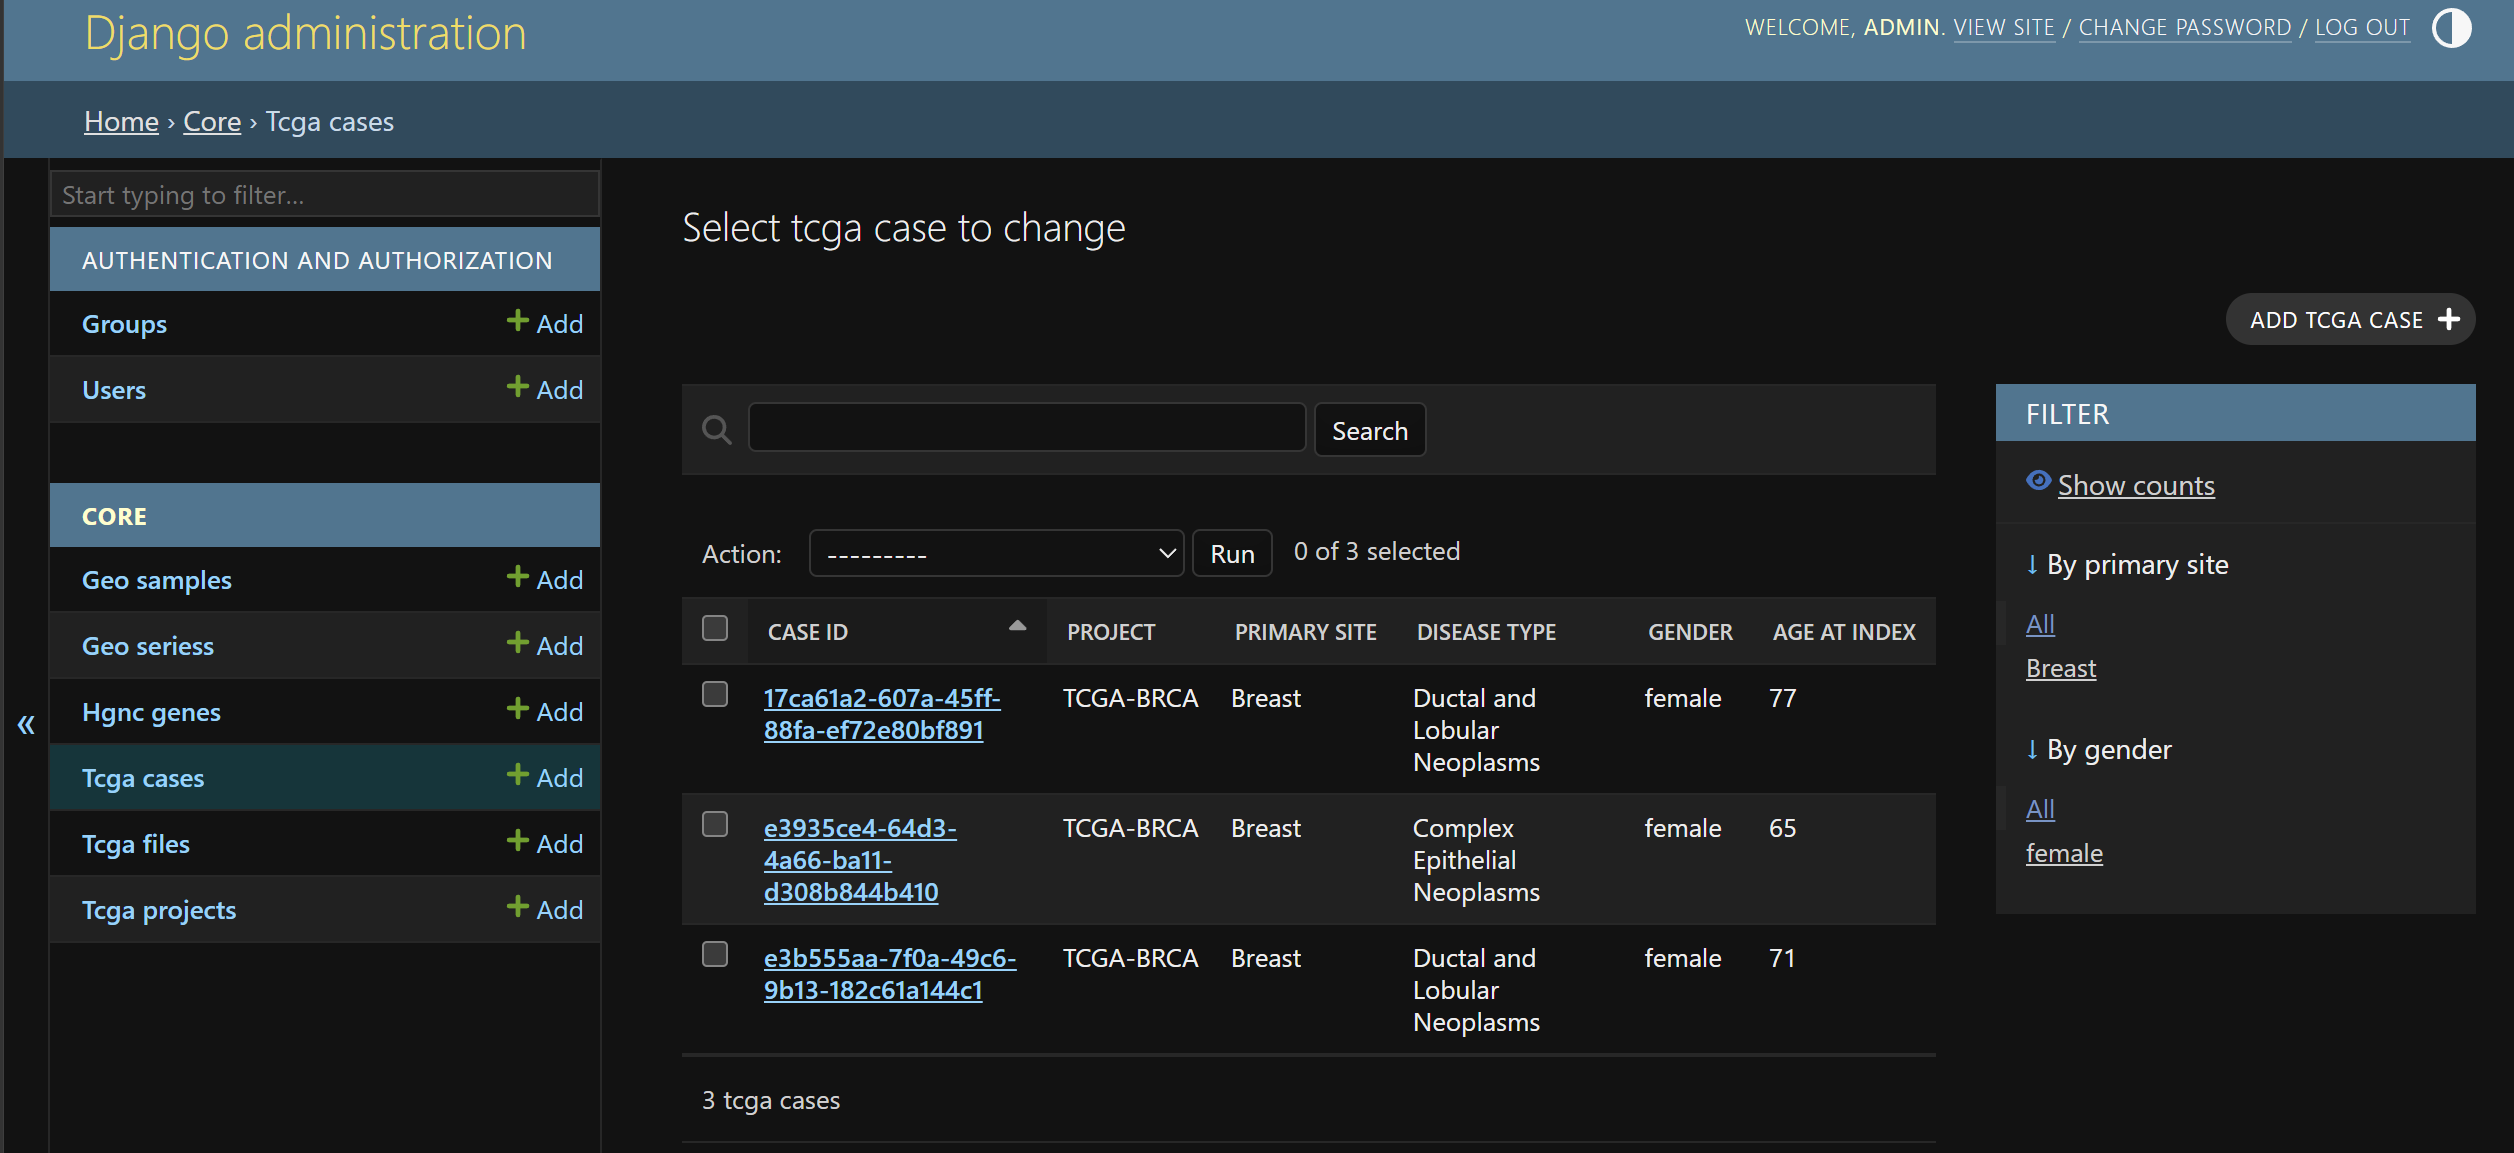
\includegraphics[width=0.9\textwidth]{img/django-admin-tcgacase.png}
\caption[Metadatos clínicos de TCGA-BRCA en el panel de administración de Django.]{Muestra de metadatos clínicos de TCGA-BRCA almacenados en la base de datos y visibles desde el panel de administración de Django.}
\label{fig:admin2}
\end{figure}

Además del panel de administración, la aplicación web ofrece una vista propia de integración. En la ruta principal (\texttt{/}), el usuario busca un gen por su símbolo y obtiene, en una sola pantalla, sus metadatos de HGNC (nombre, identificadores de Entrez y Ensembl y alias), sus registros de mutaciones y sus valores de expresión en TCGA. Los resultados se pueden filtrar por proyecto, tipo de variante, TPM mínimo, FPKM-UQ mínimo y número de filas, y se pueden exportar a CSV, XLSX o ZIP (figura~\ref{fig:webapp}). El panel de administración (\texttt{/admin/}), por su parte, permite consultar y filtrar cada una de las tablas del modelo de datos, incluidos los resultados del clasificador.

\begin{figure}[htbp]
\centering
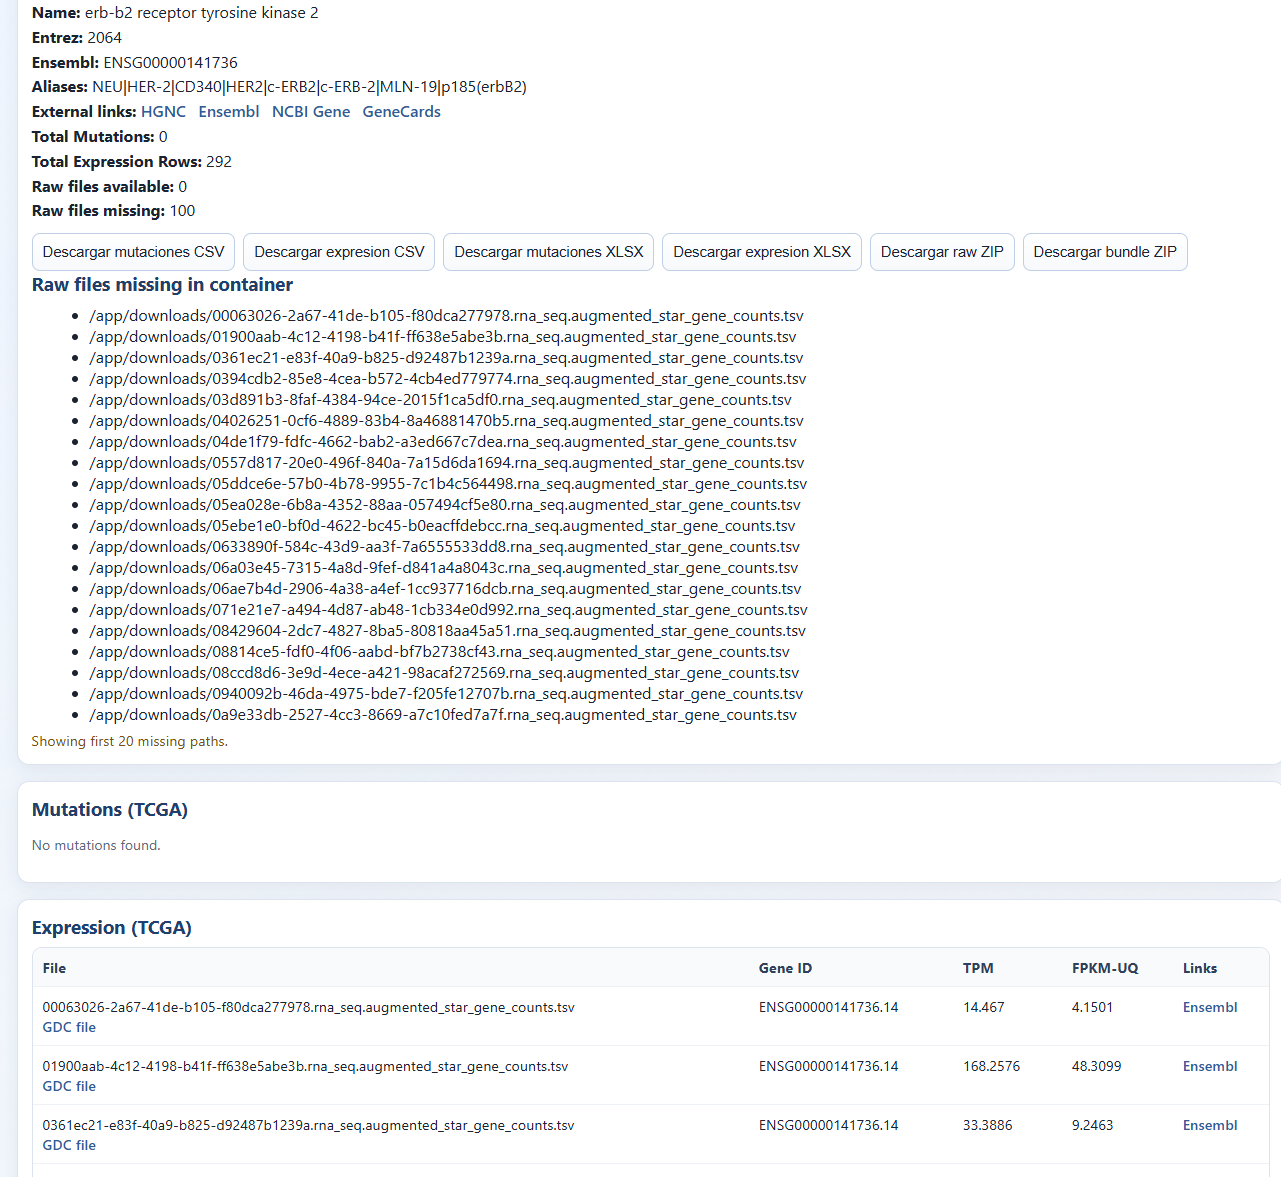
\includegraphics[width=0.8\textwidth]{img/webapp_gene_erbb2_2.png}
\caption[Vista integrada de gen de la aplicación web.]{Vista integrada de gen de la aplicación web: para el gen ERBB2 muestra sus metadatos de HGNC y los valores de expresión (TPM) en las muestras de TCGA, junto con opciones de exportación.}
\label{fig:webapp}
\end{figure}

\section{Conjunto de datos para clasificación PAM50}

De los 843 casos con etiqueta PAM50, 221 disponen de fichero TSV de expresión génica descargado localmente, que es el subconjunto utilizable para el análisis de clasificación. La distribución de subtipos en ese subconjunto se recoge en la tabla~\ref{tab:pam50_dist}.

\begin{table}[htbp]
\caption{Distribución de subtipos PAM50 en el subconjunto de 221 casos con expresión génica disponible localmente.}
\label{tab:pam50_dist}
\centering
\begin{tabular}{lrr}
\toprule
\textbf{Subtipo PAM50} & \textbf{N} & \textbf{\%} \\
\midrule
LumA   & 106 & 48{,}0 \\
LumB   &  39 & 17{,}6 \\
Basal  &  31 & 14{,}0 \\
Normal &  30 & 13{,}6 \\
Her2   &  15 &  6{,}8 \\
\midrule
\textbf{Total} & \textbf{221} & \textbf{100} \\
\bottomrule
\end{tabular}
\end{table}

La figura~\ref{fig:dist_pam50} compara la distribución de subtipos en ambas cohortes: mientras que en TCGA-BRCA la clase mayoritaria es LumA, en GSE25055 lo es Basal.

\begin{figure}[htbp]
\centering
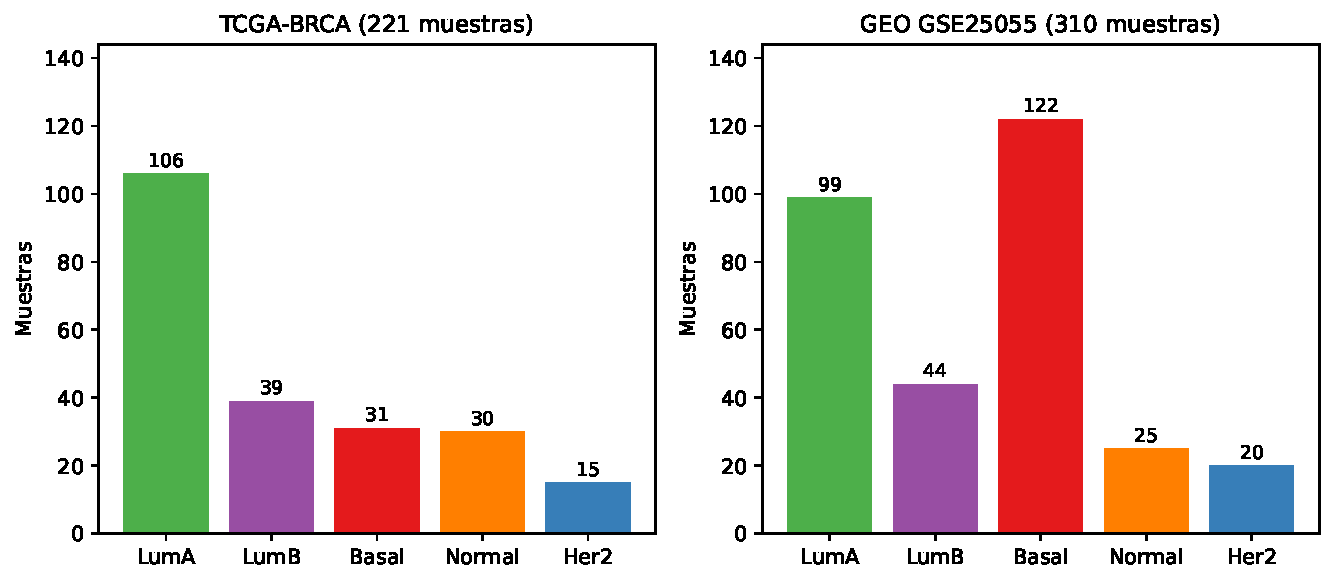
\includegraphics[width=0.95\textwidth]{figures_nuevas/distribucion_pam50.pdf}
\caption[Distribución de subtipos PAM50 en TCGA-BRCA y GSE25055.]{Distribución de subtipos PAM50 en el subconjunto de 221 muestras de TCGA-BRCA (izquierda) y en las 310 muestras de GEO GSE25055 (derecha).}
\label{fig:dist_pam50}
\end{figure}

La figura~\ref{fig:pca_pam50} muestra la PCA de las 221 muestras TCGA-BRCA coloreadas por subtipo PAM50, usando los 3000 genes seleccionados. Hay solapamiento en prácticamente todos los subtipos; esto significa que el modelo tendrá que buscar patrones complejos para distinguirlos.

\begin{figure}[htbp]
\centering
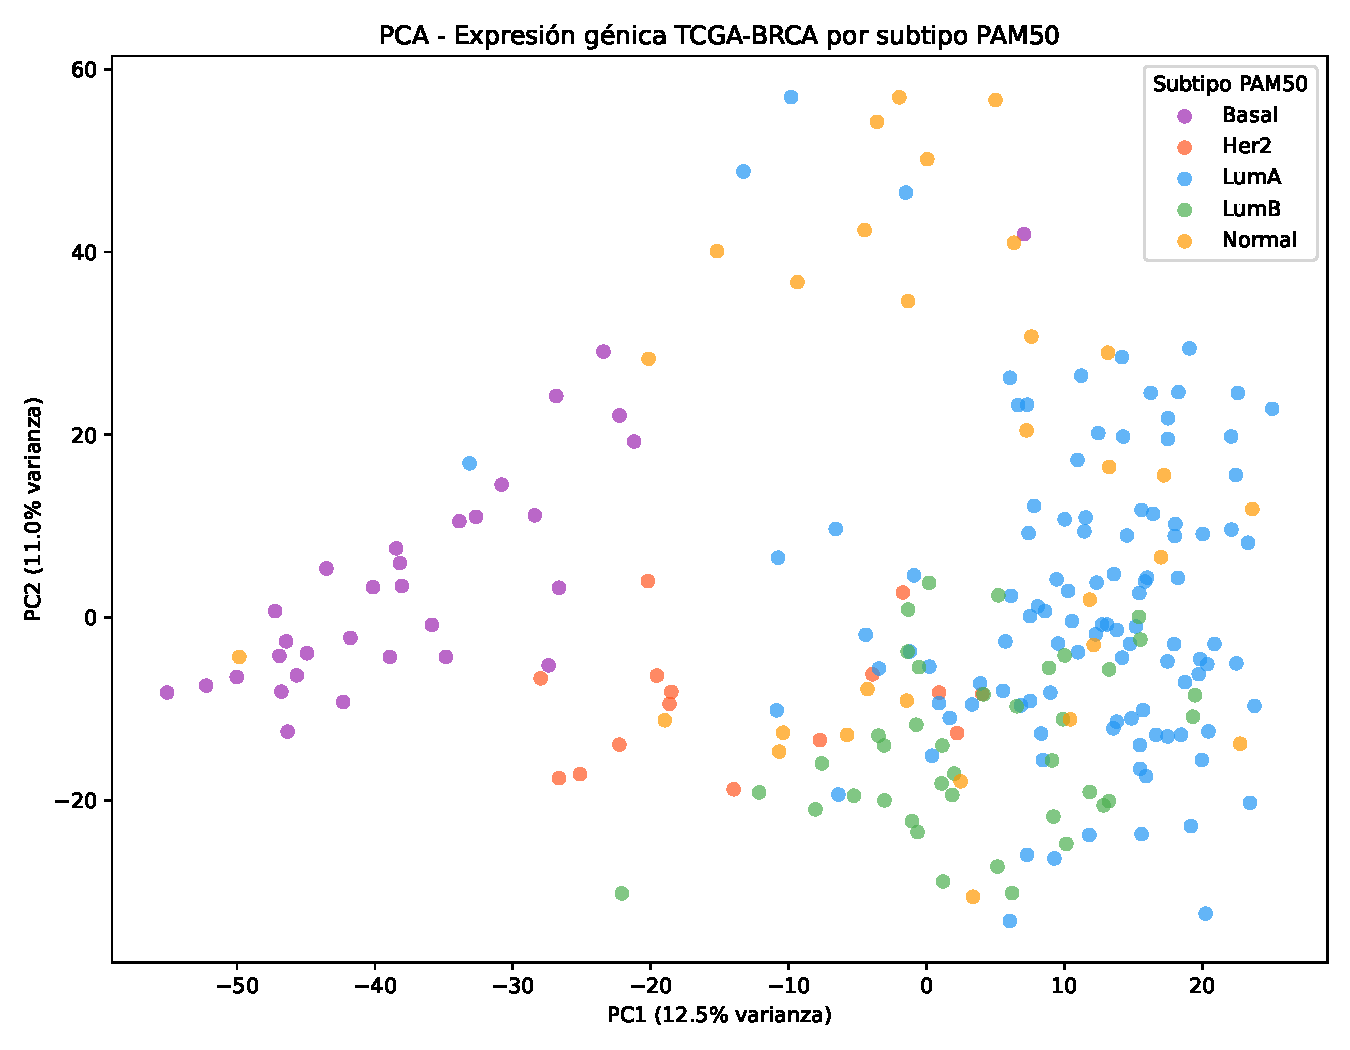
\includegraphics[width=0.85\textwidth]{figures/pca_pam50.pdf}
\caption[PCA de las 221 muestras TCGA-BRCA por subtipo PAM50.]{Proyección de las dos primeras componentes principales de las 221 muestras TCGA-BRCA, coloreadas por subtipo PAM50.}
\label{fig:pca_pam50}
\end{figure}

\section{Entrenamiento y validación interna TCGA-BRCA}

El clasificador Random Forest se entrenó sobre las 221 muestras TCGA-BRCA con etiqueta PAM50 usando los 3000 genes de mayor varianza. Al probarlo con 45 muestras que no había visto (20\% del total), acertó el 68,9\% de las veces (\textit{accuracy}). El F1 macro sobre el conjunto de test fue de 0,633 y el AUC macro (cada subtipo contra el resto) de 0,858; en la validación cruzada de 5 pliegues el F1 macro medio fue de 0,701 $\pm 0,108$.

La tabla~\ref{tab:internal_metrics} desglosa las métricas por subtipo sobre el conjunto de test interno.

\begin{table}[htbp]
\caption{Métricas por subtipo del clasificador Random Forest en la validación interna (45 muestras de test de TCGA-BRCA).}
\label{tab:internal_metrics}
\centering
\begin{tabular}{lrrrr}
\toprule
\textbf{Subtipo} & \textbf{Precision} & \textbf{Recall} & \textbf{F1} & \textbf{Support} \\
\midrule
Basal  & 1{,}00 & 1{,}00 & 1{,}00 &  6 \\
Her2   & 0{,}60 & 1{,}00 & 0{,}75 &  3 \\
LumA   & 0{,}83 & 0{,}68 & 0{,}75 & 22 \\
LumB   & 0{,}54 & 0{,}88 & 0{,}67 &  8 \\
Normal & 0{,}00 & 0{,}00 & 0{,}00 &  6 \\
\midrule
Macro avg    & 0{,}59 & 0{,}71 & 0{,}63 & 45 \\
Weighted avg & 0{,}68 & 0{,}69 & 0{,}67 & 45 \\
\midrule
\multicolumn{4}{l}{\textbf{Accuracy}} & \textbf{0{,}69} \\
\bottomrule
\end{tabular}
\end{table}

La figura~\ref{fig:cm_internal} muestra la matriz de confusión sobre el conjunto de test interno y la figura~\ref{fig:roc_internal} las curvas ROC por subtipo. En ellas se aprecia que las clases mejor separadas son Basal, Her2 y LumA (AUC entre 0,92 y 1,00), mientras que Normal apenas supera el azar (AUC 0,49), coherente con que ninguna de sus 6 muestras se clasificó bien. La figura~\ref{fig:fi_rf} recoge los 20 genes con mayor importancia según el modelo entrenado.

Los veinte genes con mayor importancia, con enlace a su ficha en GeneCards, se recogen en la tabla~\ref{tab:top_genes}.

\begin{table}[htbp]
\caption{Los 20 genes con mayor importancia según el clasificador Random Forest entrenado sobre TCGA-BRCA, con su nombre oficial HGNC.}
\label{tab:top_genes}
\centering
\begin{tabular}{lll}
\toprule
\textbf{Gen} & \textbf{Importancia} & \textbf{Nombre HGNC} \\
\midrule
\href{https://www.genecards.org/card/RGMA}{RGMA} & 0{,}0063 & repulsive guidance molecule BMP co-receptor a \\
\href{https://www.genecards.org/card/ROPN1}{ROPN1} & 0{,}0061 & rhophilin associated tail protein 1 \\
\href{https://www.genecards.org/card/AURKA}{AURKA} & 0{,}0056 & aurora kinase A \\
\href{https://www.genecards.org/card/ZNF552}{ZNF552} & 0{,}0055 & zinc finger protein 552 \\
\href{https://www.genecards.org/card/CCDC170}{CCDC170} & 0{,}0054 & coiled-coil domain containing 170 \\
\href{https://www.genecards.org/card/NXNL2}{NXNL2} & 0{,}0054 & nucleoredoxin like 2 \\
\href{https://www.genecards.org/card/SCUBE2}{SCUBE2} & 0{,}0053 & signal peptide, CUB domain and EGF like domain containing 2 \\
\href{https://www.genecards.org/card/TBC1D9}{TBC1D9} & 0{,}0052 & TBC1 domain family member 9 \\
\href{https://www.genecards.org/card/AGR3}{AGR3} & 0{,}0048 & anterior gradient 3, protein disulphide isomerase family member \\
\href{https://www.genecards.org/card/NAGS}{NAGS} & 0{,}0046 & N-acetylglutamate synthase \\
\href{https://www.genecards.org/card/GRB7}{GRB7} & 0{,}0046 & growth factor receptor bound protein 7 \\
\href{https://www.genecards.org/card/CDKN3}{CDKN3} & 0{,}0046 & cyclin dependent kinase inhibitor 3 \\
\href{https://www.genecards.org/card/FOXC1}{FOXC1} & 0{,}0045 & forkhead box C1 \\
\href{https://www.genecards.org/card/ESR1}{ESR1} & 0{,}0042 & estrogen receptor 1 \\
\href{https://www.genecards.org/card/HJURP}{HJURP} & 0{,}0041 & Holliday junction recognition protein \\
\href{https://www.genecards.org/card/XBP1}{XBP1} & 0{,}0039 & X-box binding protein 1 \\
\href{https://www.genecards.org/card/MLPH}{MLPH} & 0{,}0039 & melanophilin \\
\href{https://www.genecards.org/card/STARD3}{STARD3} & 0{,}0039 & StAR related lipid transfer domain containing 3 \\
\href{https://www.genecards.org/card/FOXA1}{FOXA1} & 0{,}0038 & forkhead box A1 \\
\href{https://www.genecards.org/card/CHAC1}{CHAC1} & 0{,}0037 & ChaC glutathione specific gamma-glutamylcyclotransferase 1 \\
\midrule
\end{tabular}
\end{table}

\begin{figure}[htbp]
\centering
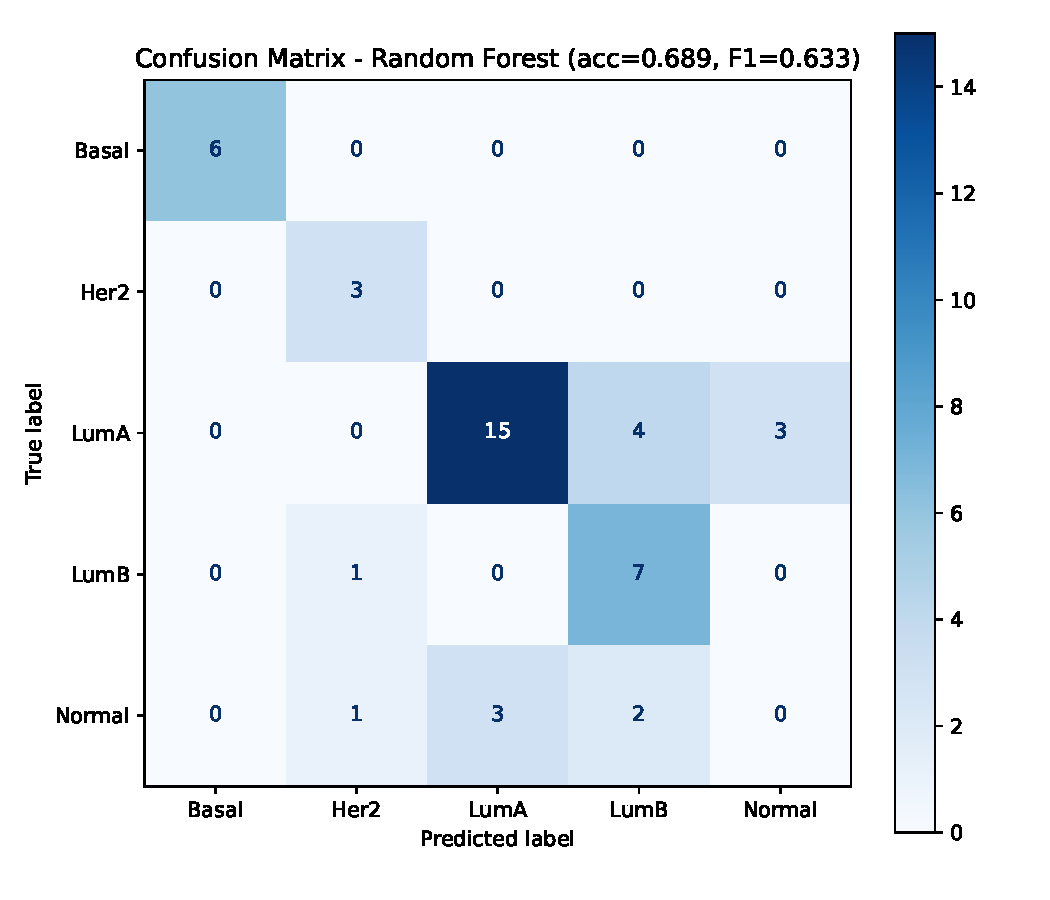
\includegraphics[width=0.78\textwidth]{figures/confusion_matrix_rf.pdf}
\caption[Matriz de confusión en validación interna]{Matriz de confusión sobre las 45 muestras de test de TCGA-BRCA}
\label{fig:cm_internal}
\end{figure}

\begin{figure}[htbp]
\centering
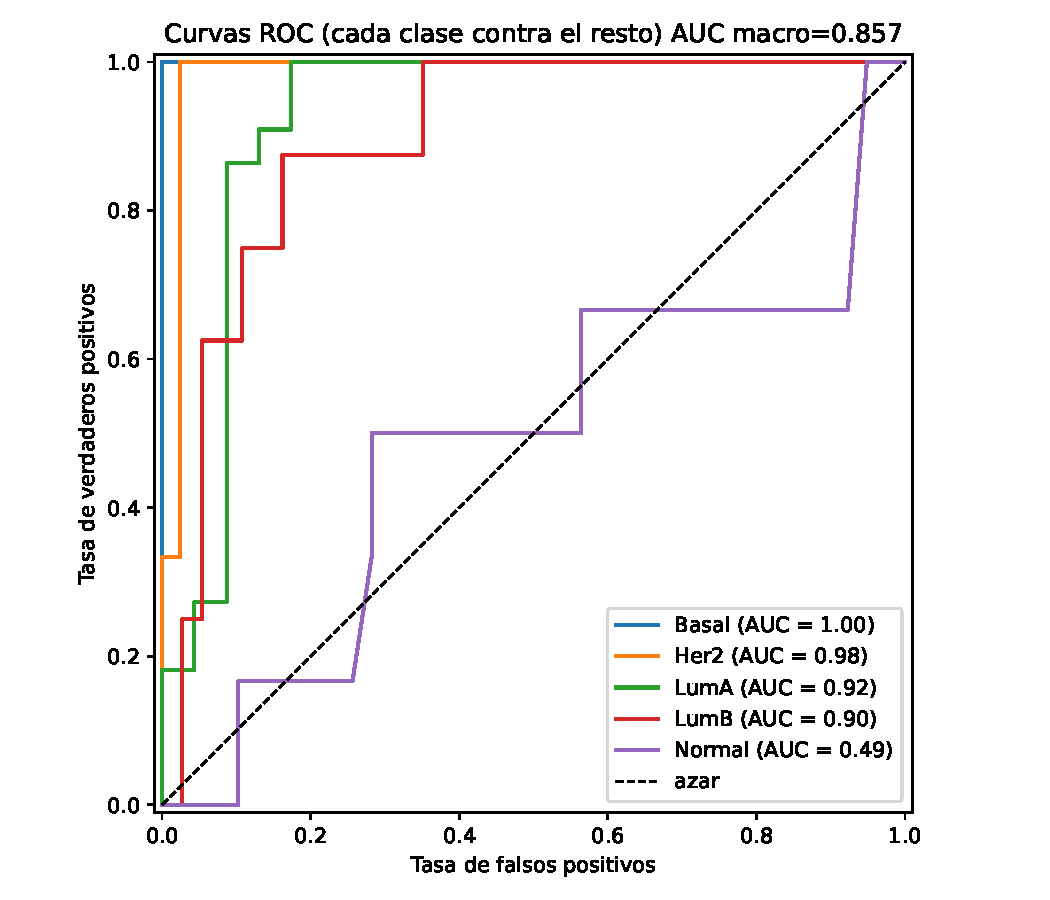
\includegraphics[width=0.78\textwidth]{figures/roc_curves_rf.pdf}
\caption[Curvas ROC en validación interna.]{Curvas ROC por subtipo (uno contra el resto) sobre el conjunto de test interno de TCGA-BRCA. La línea discontinua representa el azar.}
\label{fig:roc_internal}
\end{figure}

\begin{figure}[htbp]
\centering
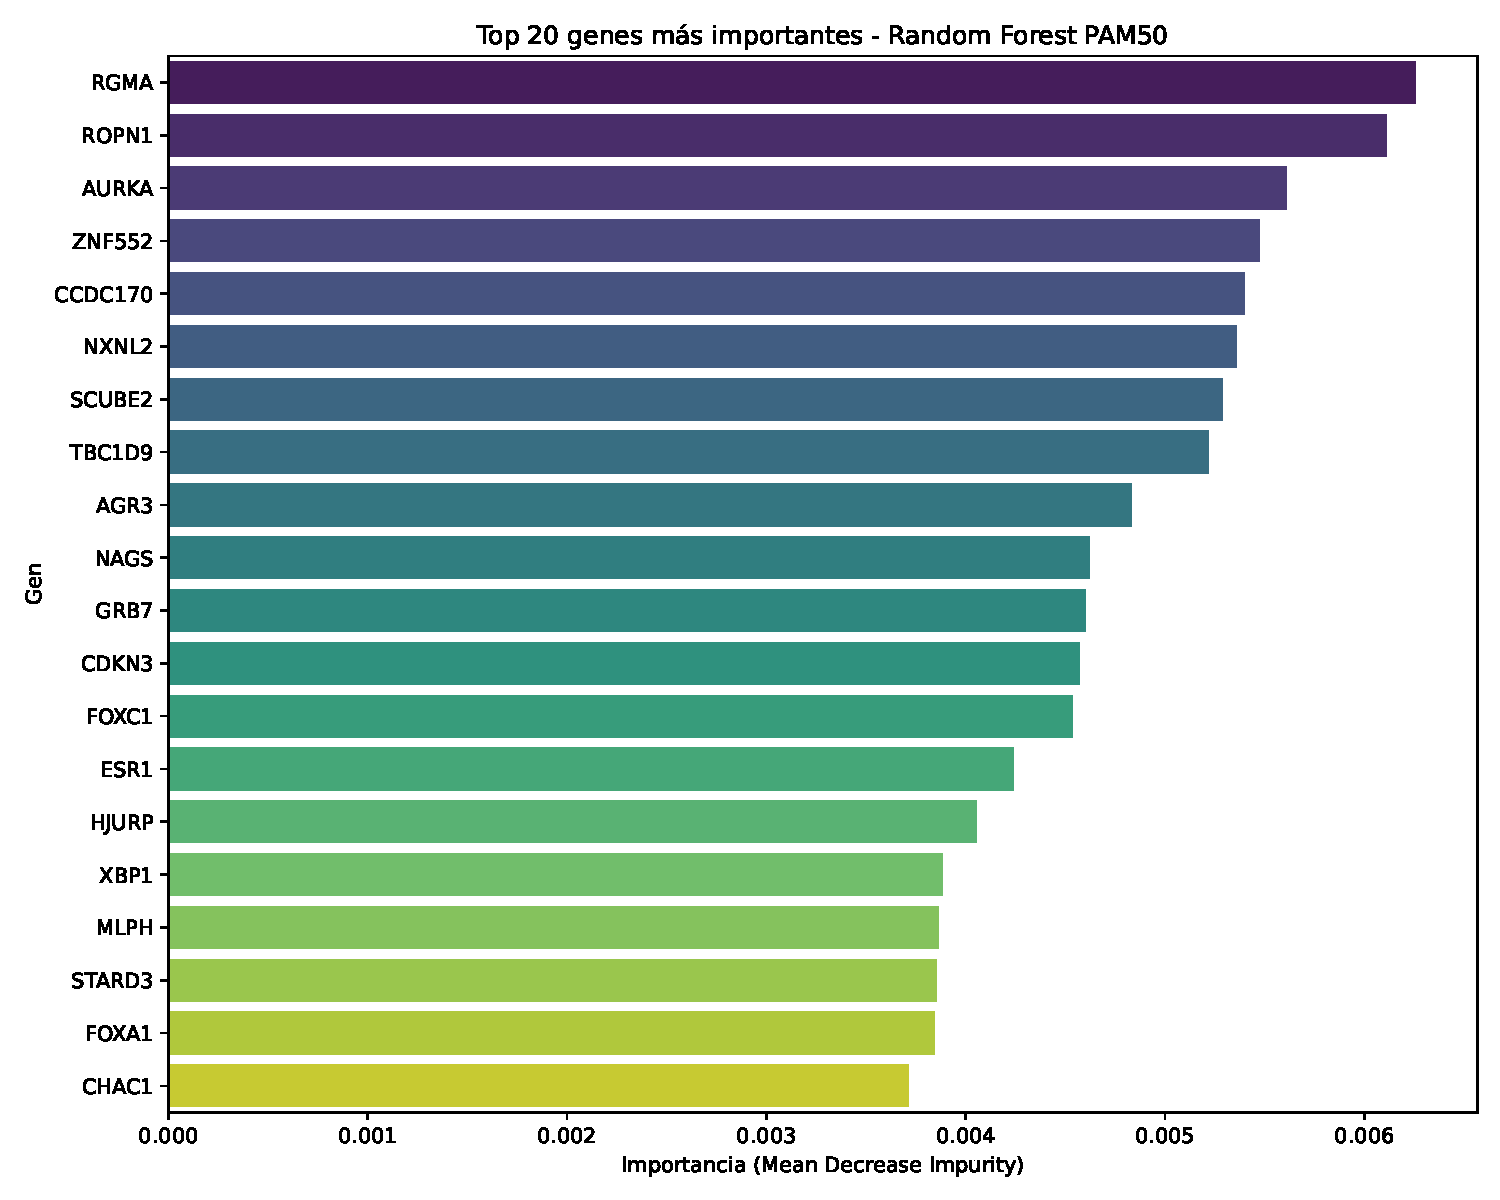
\includegraphics[width=0.85\textwidth]{figures/feature_importances_rf.pdf}
\caption[Importancia de los 20 genes más relevantes (Random Forest).]{Los 20 genes con mayor importancia según el clasificador Random Forest entrenado sobre TCGA-BRCA.}
\label{fig:fi_rf}
\end{figure}

Los resultados del modelo quedan almacenados en la base de datos y son consultables desde el panel de administración (figuras~\ref{fig:admin_mlrun} y \ref{fig:admin_mlgenes}).

\begin{figure}[htbp]
\centering
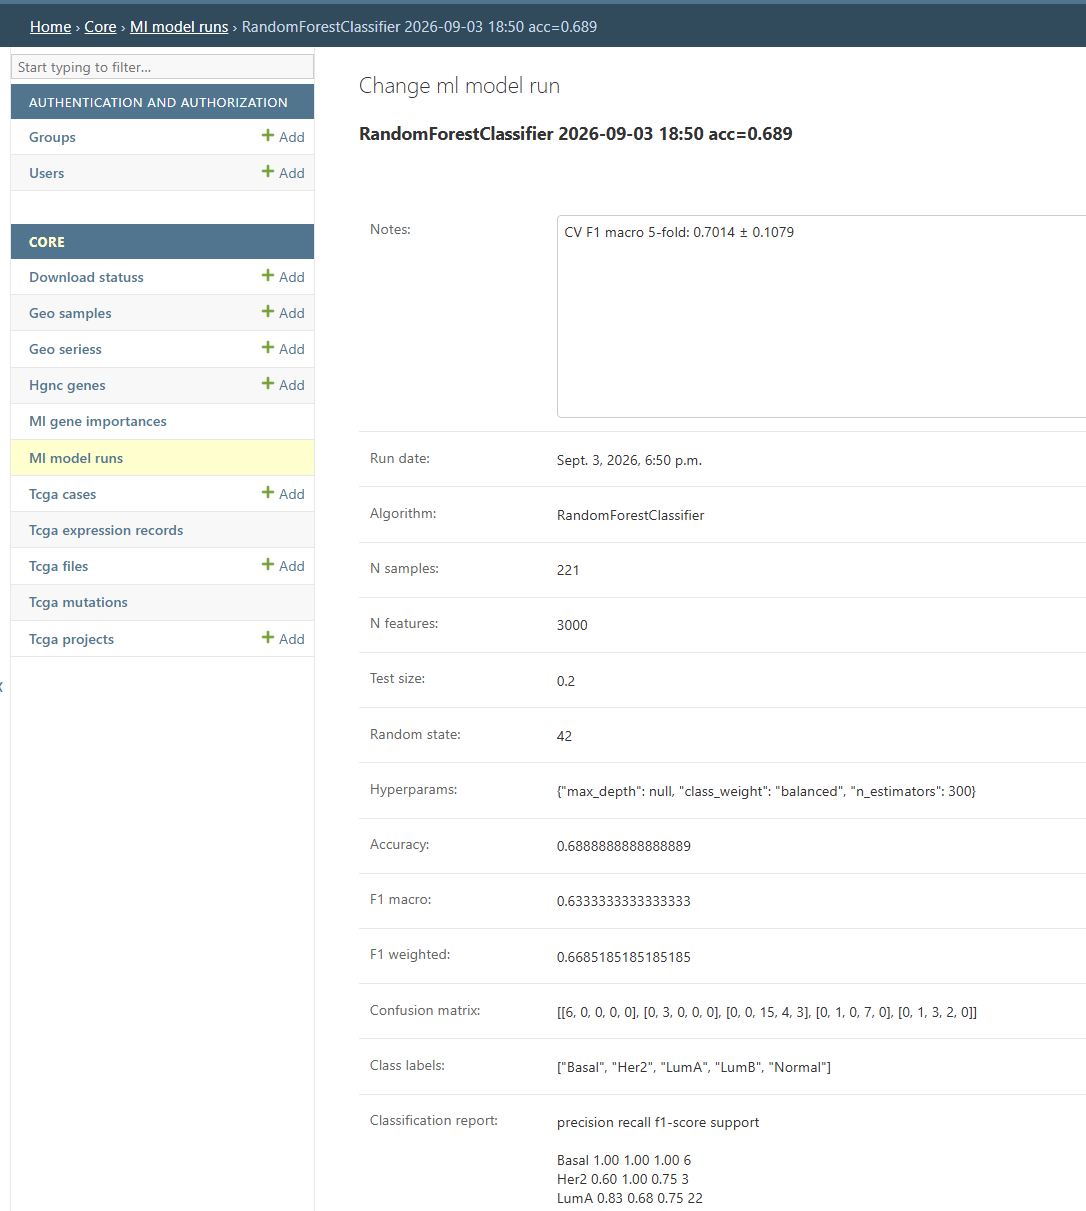
\includegraphics[width=0.85\textwidth]{img/admin-mlmodelrun.png}
\caption[Registro del modelo en el panel de administración.]{Ficha del registro del modelo en el panel de administración de Django, con la exactitud, el F1, la matriz de confusión y el informe de clasificación.}
\label{fig:admin_mlrun}
\end{figure}

\begin{figure}[htbp]
\centering
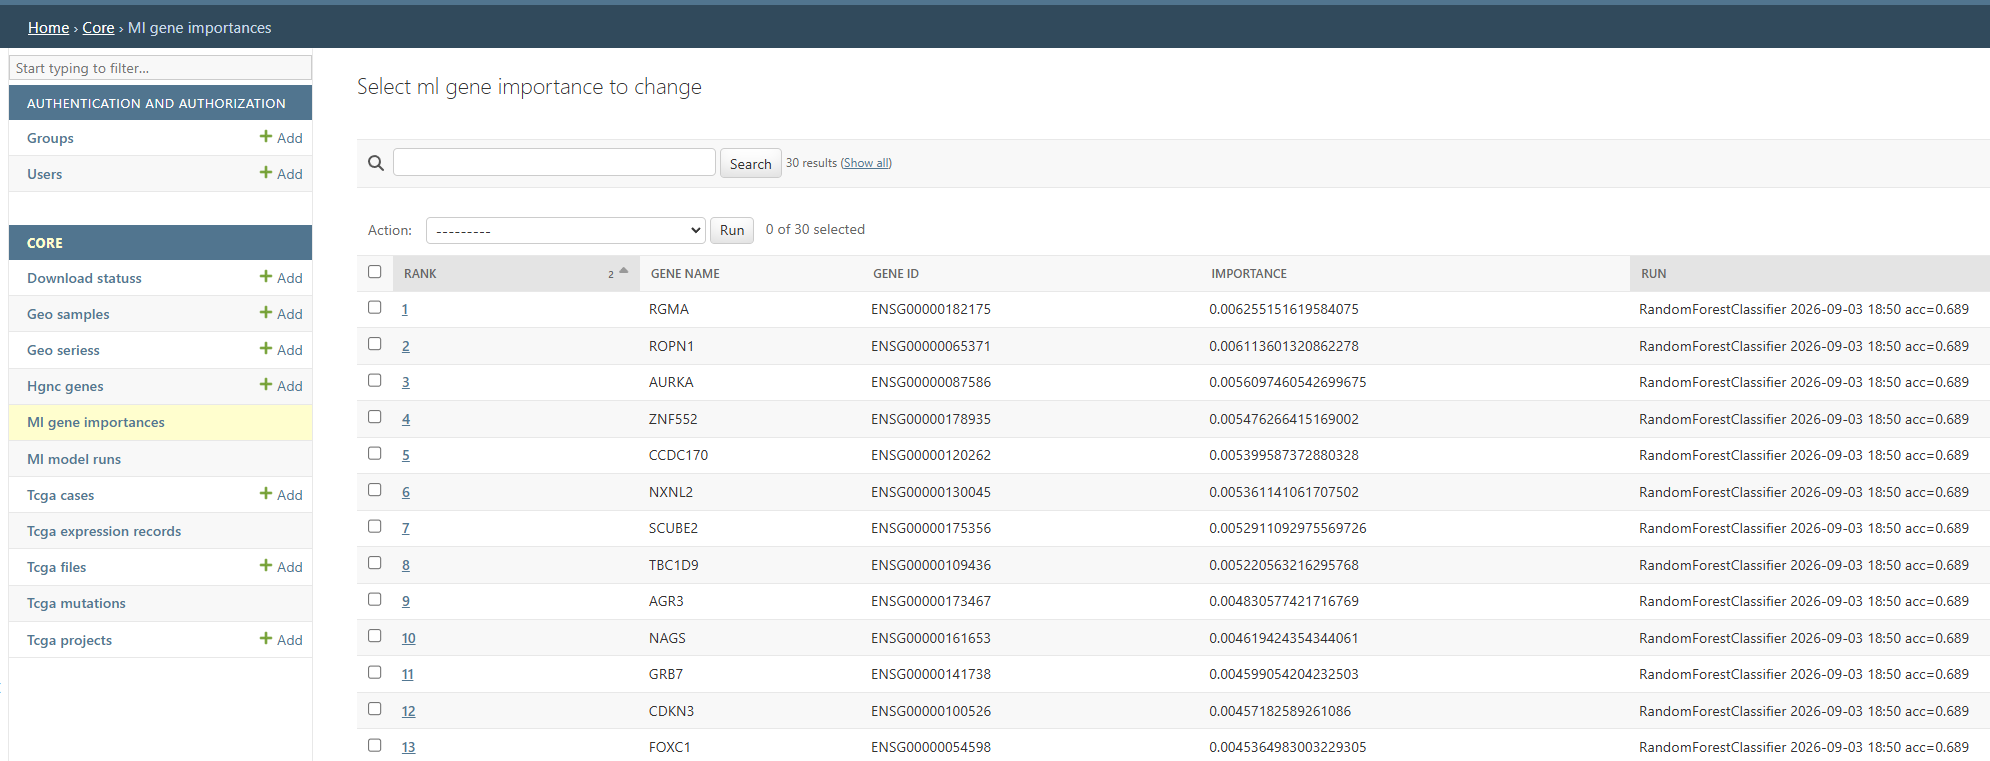
\includegraphics[width=0.85\textwidth]{img/admin-mlgeneimportance.png}
\caption[Importancia de los genes en el panel de administración.]{Ranking de importancia de los genes almacenado en la base de datos y visible desde el panel de administración de Django.}
\label{fig:admin_mlgenes}
\end{figure}

\section{Validación cross-platform: TCGA \texorpdfstring{$\rightarrow$}{->} GEO GSE25055}

El modelo entrenado con TCGA se aplicó directamente sobre 310 muestras de GEO GSE25055, sin reentrenar ni ajustar. La \textit{accuracy} cayó al 61,0\%, 7,9 puntos por debajo del rendimiento interno, y el F1 macro bajó a 0,457. El AUC macro (cada subtipo contra el resto), en cambio, se mantuvo alto (0,892).

La tabla~\ref{tab:cross_metrics} desglosa las métricas por subtipo. De los 3000 genes seleccionados en TCGA, 2193 (73,1\%) están disponibles en la plataforma de microarray de GEO, los 807 restantes se imputan con valor 0, equivalente a expresión media en z-score.

\begin{itemize}
  \item \textbf{Basal}: precisión perfecta (1,00) con recall moderado (0,49). El modelo no confunde otros subtipos con Basal, pero solo encuentra la mitad de los Basales reales.
  \item \textbf{LumA}: recall perfecto (1,00) pero precisión moderada (0,52). El modelo encuentra todos los LumA reales, pero casi la mitad de sus predicciones de LumA corresponden a otras clases. LumA es la segunda clase más numerosa (99 de 310).
  \item \textbf{Her2}: precisión perfecta (1,00) pero recall muy bajo (0,10): solo detecta 1 de cada 10 Her2 reales. Es el subtipo más pequeño (20 muestras) y el que menos solapamiento tiene entre plataformas.
  \item \textbf{LumB}: precisión y recall equilibrados en torno a 0,52--0,55, el subtipo minoritario mejor clasificado.
  \item \textbf{Normal}: el peor clasificado (F1 de 0,23), con la mayoría de sus muestras asignadas a otras clases.
\end{itemize}

Esta evaluación se ejecuta desde el python notebook \texttt{cross\_validation.ipynb}.

La figura~\ref{fig:cm_cross} muestra la matriz de confusión y la figura~\ref{fig:comparison} compara las métricas globales entre las dos condiciones de evaluación.

\begin{table}[htbp]
\caption{Métricas del clasificador Random Forest por subtipo PAM50 en el conjunto de test cross-platform (310 muestras GEO GSE25055).}
\label{tab:cross_metrics}
\centering
\begin{tabular}{lrrrr}
\toprule
\textbf{Subtipo} & \textbf{Precision} & \textbf{Recall} & \textbf{F1} & \textbf{Support} \\
\midrule
Basal  & 1{,}00 & 0{,}49 & 0{,}66 & 122 \\
Her2   & 1{,}00 & 0{,}10 & 0{,}18 &  20 \\
LumA   & 0{,}52 & 1{,}00 & 0{,}68 &  99 \\
LumB   & 0{,}52 & 0{,}55 & 0{,}53 &  44 \\
Normal & 0{,}40 & 0{,}16 & 0{,}23 &  25 \\
\midrule
Macro avg    & 0{,}69 & 0{,}46 & 0{,}46 & 310 \\
Weighted avg & 0{,}73 & 0{,}61 & 0{,}58 & 310 \\
\midrule
\multicolumn{4}{l}{\textbf{Accuracy}} & \textbf{0{,}61} \\
\bottomrule
\end{tabular}
\end{table}

\begin{figure}[htbp]
\centering
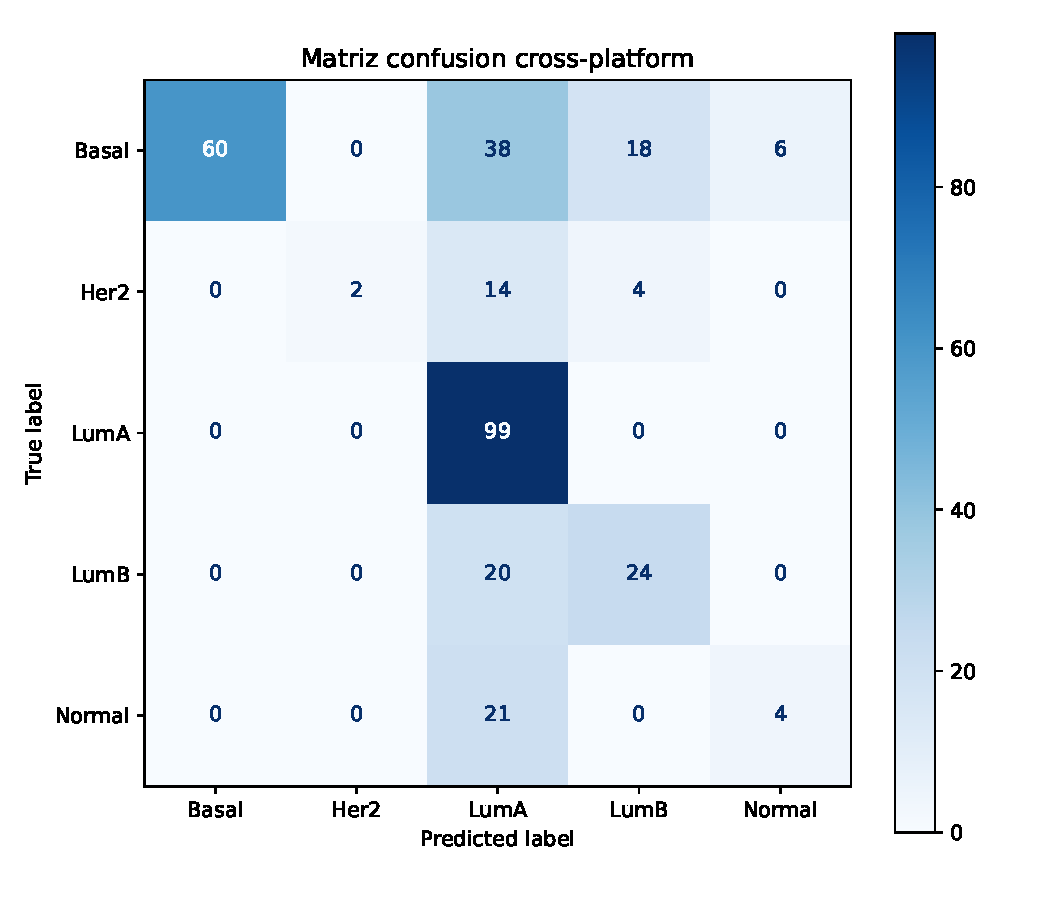
\includegraphics[width=0.78\textwidth]{figures/confusion_matrix_crossplatform.pdf}
\caption[Matriz de confusión cross-platform (TCGA $\rightarrow$ GEO GSE25055).]{Matriz de confusión sobre las 310 muestras de GEO GSE25055. El modelo tiende a clasificar la mayoría de las muestras como LumA (recall = 1,00), mientras que Basal mantiene una precisión perfecta. Her2 se detecta raramente (recall = 0,10).}
\label{fig:cm_cross}
\end{figure}

\begin{figure}[htbp]
\centering
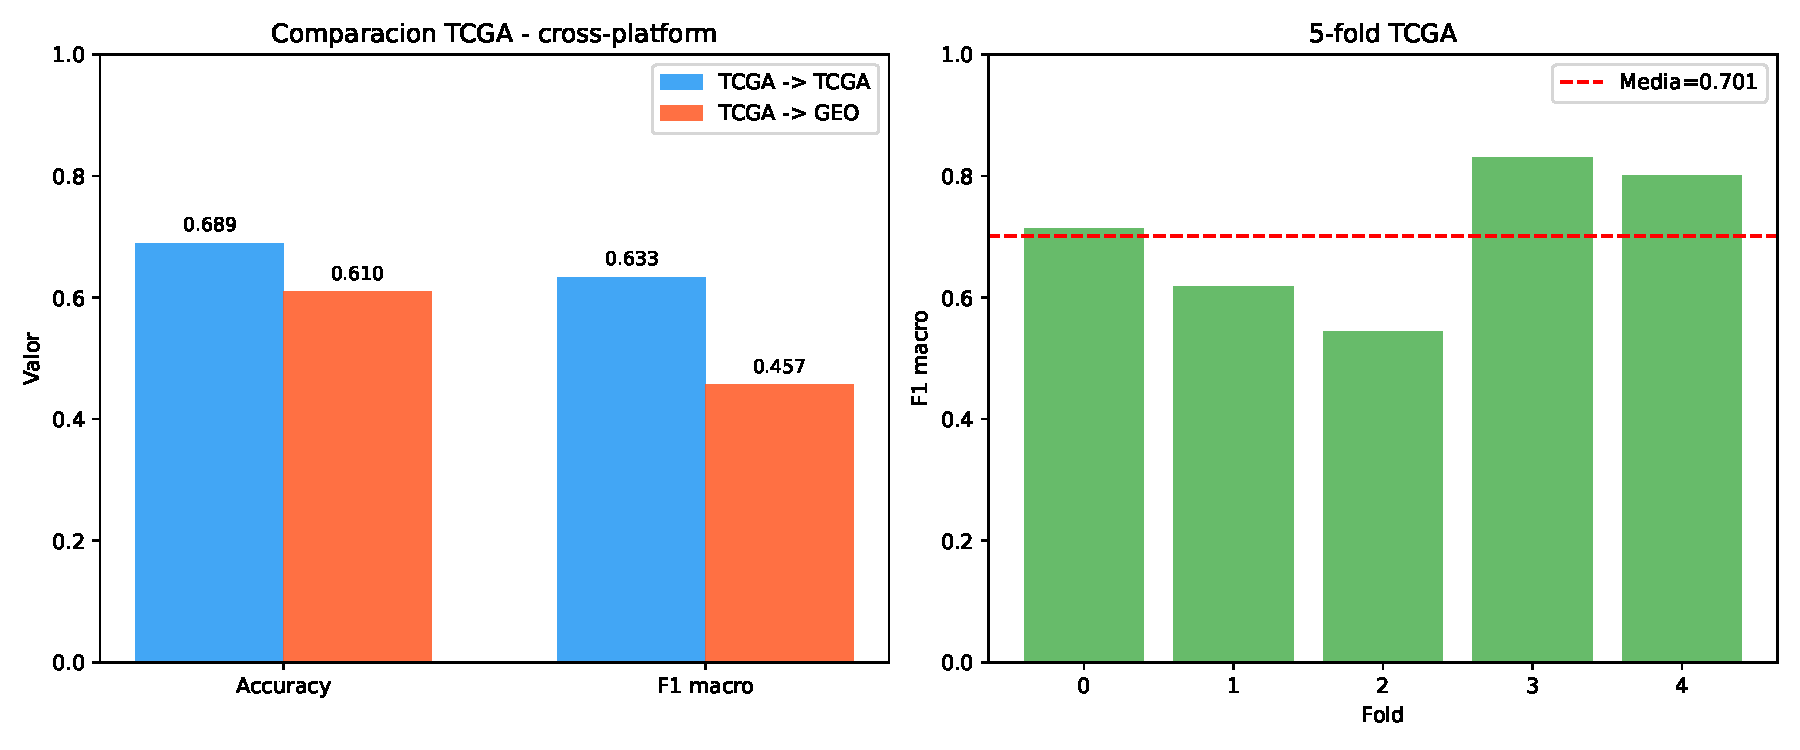
\includegraphics[width=0.95\textwidth]{figures/crossplatform_comparison.pdf}
\caption[Comparación de rendimiento TCGA-only vs.\ cross-platform.]{Izquierda: accuracy y F1 macro en evaluación interna (TCGA) y cross-platform (GEO). Derecha: F1 macro por pliegue en la validación cruzada 5-fold sobre TCGA.}
\label{fig:comparison}
\end{figure}

% ============================================================
% CAPÍTULO 5 DISCUSIÓN
% ============================================================

\chapter{Discusión}

\section{Rendimiento del clasificador PAM50}

Evaluado sobre la misma plataforma (TCGA, partición 80/20), el clasificador Random Forest alcanzó una \textit{accuracy} del 68,9\% y un F1 macro de 0,633. La validación cruzada de 5 pliegues arrojó 0,701 $\pm 0,108$, coherente con el resultado del test y confirmando que el modelo clasifica PAM50 en datos RNA-seq \cite{sorlie_gene_2001}.

Existe una alta variabilidad en la validación cruzada ($\pm 0,108$) seguramente se debe al pequeño tamaño del conjunto (221 casos): con tan pocos ejemplos de Her2 (15 casos) y Normal (30) el resultado de cada pliegue depende mucho de qué muestras caen en test. La clase Normal es la más difícil: en el test interno el modelo no acertó ninguna de sus 6 muestras (F1 = 0,00), asignándolas sobre todo a LumA. Es coherente con que sea una de las clases con menos muestras (30 de 221) y con su comportamiento en la validación cross-platform, donde también es la peor clasificada. La literatura ha descrito además que la contaminación por tejido normal no tumoral en la muestra es una fuente de sesgo que provoca errores de clasificación en los predictores genómicos, incluido PAM50 \cite{elloumi_systematic_2011}.

La composición de los genes más importantes apoya además la interpretación biológica del modelo: varios de ellos ya se asocian con los subtipos PAM50 en la literatura. AURKA interviene en la división celular, de modo que su presencia encaja con que los tumores que se dividen más (más agresivos) se distingan de los menos agresivos \cite{ali_aurora_2012, sorlie_gene_2001, parker_supervised_2009}. GRB7 y STARD3 se encuentran en la misma zona del genoma que ERBB2 \cite{kauraniemi_erbb2_2001}, el gen que da nombre al subtipo HER2-enriquecido y que es una de las dianas de tratamiento más conocidas en el cáncer de mama \cite{slamon_human_1987}. FOXA1 y ESR1 están ligados a los receptores de estrógenos, típicos de los tumores luminales \cite{seachrist_foxa1_2021}. Por último, FOXC1 se asocia al subtipo basal, en el que se ha descrito como marcador con valor pronóstico y funcional \cite{ray_foxc1_2010}.

\section{Efecto del cambio de plataforma tecnológica}

La caída de 7,9 puntos de \textit{accuracy} al pasar de TCGA a GEO muestra que el modelo entrenado en RNA-seq pierde algo de rendimiento con datos de microarray, aunque se mantiene muy por encima del azar. Basal mantiene precisión perfecta (1,00), lo que indica que es lo bastante distinto para ser detectado incluso con otra tecnología. Her2, en cambio, apenas se detecta (recall de 0,10) pese a que sus pocas predicciones son correctas. LumA, la segunda clase más numerosa (99 de 310), recibe casi todas las predicciones (recall = 1,00), pero a costa de una precisión moderada (0,52). Pese a esta caída, el AUC macro (cada subtipo contra el resto) se mantuvo alto (0,892 frente a 0,858 en la validación interna), lo que indica que el modelo conserva la capacidad de ordenar las muestras por probabilidad de pertenencia a cada subtipo: la pérdida se concentra en la decisión final de asignación, no en la discriminación.

Esta caída se puede descomponer en dos factores. El primero es el solapamiento génico: 2193 de los 3000 genes seleccionados (73,1\%) están presentes en la plataforma de microarray, y el 26,9\% restante se imputa a cero, lo que elimina parte de la señal sobre la que se entrenó el modelo. El segundo es el desequilibrio de clases entre cohortes: en TCGA la clase mayoritaria es LumA (48\% de las 221 muestras), mientras que en GSE25055 lo es Basal (39\% de las 310), de modo que la distribución sobre la que se evalúa el modelo es distinta a la del entrenamiento.

Este resultado es coherente con la literatura sobre la sensibilidad de la firma PAM50 al cambio de plataforma: cuando la firma se mide sobre las mismas muestras con dos tecnologías distintas, la concordancia entre plataformas es alta \cite{picornell_breast_2019}. En este trabajo, sin embargo, el modelo cruza además distintos pacientes y distintas cohortes, lo que añade una fuente adicional de variación y explica la caída observada.

\section{Lecciones del modelo de datos}

La decisión de usar una base de datos relacional con Django ORM en lugar de ficheros planos permitió cruzar datos de expresión con metadatos clínicos y etiquetas mediante consultas a base de datos sin cargar en memoria la totalidad de los registros. El uso de HGNC como capa de mapeo entre datos evitó depender de que GEO y TCGA compartan identificadores.

La inspección de datos reales reveló que parte de los metadatos de GEO no son columnas estables entre estudios y aparecen como texto semiestructurado. Almacenarlos en \texttt{JSONField} es útil para al menos poder acceder a ellos sin necesidad de normalizar la estructura, aunque sería preferible que los repositorios ofrecieran un formato estandarizado.

\section{Limitaciones}

La limitación principal del módulo de clasificación es el tamaño del subconjunto de entrenamiento: únicamente 221 de los 843 casos TCGA-BRCA con etiqueta PAM50 disponían de fichero TSV descargado localmente. En la validación externa, la imputación con ceros de los genes ausentes en GEO (26,9\%) seguramente perjudique a las clases minoritarias como Her2 y Normal.



% ============================================================
% CAPÍTULO 6 CONCLUSIONES
% ============================================================

\chapter{Conclusiones}

Este trabajo demuestra que es viable construir un pipeline bioinformático completo que integre datos de expresión génica de dos repositorios públicos con formatos y tecnologías distintas, almacenarlos en una base de datos relacional y utilizarlos para clasificación.

El clasificador Random Forest entrenado sobre 221 muestras TCGA-BRCA alcanza un 68,9\% de \textit{accuracy} en validación interna tras aplicar el preprocesado (log, selección de los 3000 genes más variables y z-score).

La validación cross-platform sobre 310 muestras de microarray GEO GSE25055 arrojó un 61,0\% de \textit{accuracy}, 7,9 puntos por debajo del rendimiento interno. Esta caída cuantifica el coste de cambiar de plataforma y resulta moderada, lo que indica que la señal biológica PAM50 se conserva en gran medida entre tecnologías.

\section{Cumplimiento de los objetivos}

Los seis objetivos específicos planteados al inicio se han alcanzado de la siguiente manera:

\begin{enumerate}
  \item \textbf{Análisis de herramientas}: se revisaron las soluciones existentes y se comprobó que están fragmentadas entre R y Python, sin ninguna que cubra de forma integrada las dos fuentes junto con la normalización y el almacenamiento.
  \item \textbf{Exploración de los datos}: se examinaron los datos disponibles en GEO y TCGA, confirmando que difieren en formato, tecnología e identificadores.
  \item \textbf{Estrategia de integración}: se definió un vocabulario común basado en HGNC que traduce los identificadores de ambas fuentes y permite expresar la expresión en una escala comparable.
  \item \textbf{Solución de almacenamiento}: se diseñó una base de datos relacional con el ORM de Django, capaz de cruzar expresión y metadatos clínicos y de registrar el estado de cada descarga.
  \item \textbf{Prototipo funcional}: se implementó un pipeline que descarga, parsea, integra y almacena datos de ambas fuentes, ingiriendo 17,7 millones de registros de expresión.
  \item \textbf{Capacidad predictiva}: se entrenó un clasificador supervisado que predice el subtipo PAM50 y se evaluó su comportamiento al cambiar de plataforma.
\end{enumerate}

\section{Líneas futuras}

El trabajo deja varias líneas abiertas que podrían mejorar el pipeline y sus resultados:

\begin{itemize}
  \item \textbf{Ampliar el conjunto de entrenamiento}: de los 843 casos con etiqueta PAM50, solo 221 disponían de fichero local. Descargar el resto permitiría entrenar con más muestras y reducir la variabilidad observada en la validación cruzada.
  \item \textbf{Mejorar la armonización cross-platform}: la imputación con ceros de los genes ausentes en GEO perjudica a las clases minoritarias. Podrían probarse métodos de normalización entre lotes o de imputación más elaborados.
  \item \textbf{Explorar otros modelos}: además de Random Forest, se podrían evaluar máquinas de vectores de soporte, modelos lineales regularizados o redes neuronales, y comparar su rendimiento.
  \item \textbf{Incorporar otros tipos de datos ómicos}: el modelo de datos ya contempla mutaciones, por lo que podría extenderse el análisis a otros niveles, como la metilación o la proteómica.
  \item \textbf{Empaquetar el pipeline}: convertir el prototipo en una herramienta reutilizable con una interfaz de línea de comandos clara y documentación, para facilitar su uso por otros investigadores.
  \item \textbf{Integrar los notebooks en el servicio web}: hoy el entrenamiento y la validación del clasificador se ejecutan en notebooks Jupyter externos a la aplicación. Llevarlos al propio servicio web, y documentar el acceso a los datos mediante el ORM de Django, sus tipos de consulta y la API de \textit{querysets} \cite{noauthor_making_nodate}, facilitaría reproducir el análisis sin salir de la aplicación.
  \item \textbf{Exponer una API REST}: además de la vista HTML integrada, ofrecer endpoints JSON para consultar de forma programática la expresión y las mutaciones ya integradas.
  \item \textbf{Añadir pruebas automatizadas}: cubrir conectores, parsers y comandos de gestión con tests unitarios que garanticen la estabilidad ante futuros cambios.
  \item \textbf{Control de acceso y autenticación}: proteger la vista integrada de gen y separar los roles de consulta y administración.
  \item \textbf{Ampliar a otros tipos de cáncer}: el modelo de datos es genérico y permitiría incorporar otros proyectos de TCGA o series de GEO sin modificar el esquema.
  \item \textbf{Integración continua}: automatizar con GitHub Actions la construcción de la imagen Docker y la ejecución de los tests.
\end{itemize}


% ============================================================
% ANEXOS
% ============================================================

\unnumberedchapter{Anexo A. Manual de reproducción}

El código fuente del proyecto está disponible en el repositorio público de GitHub: \url{https://github.com/dowdyph0/tfm-bio-unir}.

Para reproducir el trabajo se necesita Docker con Docker Compose y Python 3.12 con las dependencias declaradas en \texttt{src/app/requirements.txt} (Django 6.0.5, pandas, requests, GEOparse, rich y psycopg2-binary, entre otras). Los pasos para reconstruir el entorno son los siguientes:

\begin{enumerate}
  \item Levantar los contenedores: desde la carpeta \texttt{src/}, ejecutar \texttt{docker compose up -d}. Se crean dos servicios, \texttt{db} (PostgreSQL 15.3) y \texttt{app} (la aplicación Django).
  \item Aplicar las migraciones: \texttt{python manage.py migrate}.
  \item Cargar la referencia de genes: \texttt{python manage.py load\_hgnc\_local}.
  \item Poblar metadatos y etiquetas PAM50: \texttt{python manage.py populate\_pam50}.
  \item Reimportar la expresión desde ficheros locales: \texttt{python manage.py reimport\_local}.
  \item Procesar la serie GEO: \texttt{python manage.py sync\_geo}.
\end{enumerate}

El análisis de clasificación se reproduce con los dos notebooks del repositorio. El primero, \texttt{ml\_pam50\_classifier.ipynb}, realiza la clasificación interna sobre TCGA-BRCA; el segundo, \texttt{cross\_validation.ipynb}, la validación cross-platform sobre GEO GSE25055. Ambos se conectan a la base de datos mediante el ORM de Django y generan las figuras de la memoria.

\unnumberedchapter{Anexo B. Glosario de términos}

\begin{itemize}
  \item \textbf{RNA-seq}: técnica de secuenciación masiva del ARN que cuantifica la expresión génica contando las lecturas alineadas a cada gen.
  \item \textbf{Microarray}: tecnología que mide la expresión mediante la intensidad de hibridación de sondas, en escala logarítmica.
  \item \textbf{TPM} (\textit{Transcripts Per Million}): unidad de expresión normalizada por la longitud del gen y el tamaño de la librería.
  \item \textbf{FPKM}: unidad de expresión equivalente a fragmentos por kilobase por millón de lecturas.
  \item \textbf{Counts}: número bruto de lecturas asignadas a cada gen.
  \item \textbf{z-score}: transformación que expresa cada valor como el número de desviaciones típicas que se separa de la media de su gen.
  \item \textbf{PAM50}: clasificación molecular del cáncer de mama en cinco subtipos a partir de la expresión de 50 genes.
  \item \textbf{HGNC}: comité que asigna nombres y símbolos únicos a los genes humanos.
  \item \textbf{Ensembl}: base de datos de genomas que asigna identificadores estables a cada gen (formato ENSG...).
  \item \textbf{Entrez}: sistema de identificadores del NCBI.
  \item \textbf{ORM}: capa de software que mapea los objetos del código a tablas de una base de datos relacional.
  \item \textbf{JSON}: formato de texto para intercambiar datos con estructura de clave-valor.
  \item \textbf{Pipeline}: cadena de pasos automatizados que transforman los datos desde su descarga hasta su análisis.
  \item \textbf{Accuracy}: proporción de muestras clasificadas correctamente sobre el total.
  \item \textbf{Precision}: de las muestras que el modelo asigna a un subtipo, cuántas acierta.
  \item \textbf{Recall}: de las muestras que realmente son de un subtipo, cuántas encuentra el modelo.
  \item \textbf{F1}: media armónica de precision y recall; útil cuando las clases están desbalanceadas.
  \item \textbf{AUC-ROC}: área bajo la curva ROC, que mide la capacidad del modelo para separar un subtipo del resto.
  \item \textbf{Random Forest}: clasificador formado por muchos árboles de decisión cuyo resultado se promedia.
  \item \textbf{Validación cruzada}: técnica que reparte los datos en varios grupos y entrena el modelo varias veces, dejando cada vez un grupo distinto fuera para probarlo.
  \item \textbf{Cross-platform}: evaluación del modelo sobre datos de una plataforma distinta a la del entrenamiento.
  \item \textbf{FPKM-UQ}: unidad de expresión normalizada en el cuartil superior.
  \item \textbf{Docker}: plataforma para empaquetar aplicaciones en contenedores aislados y portables.
  \item \textbf{Django}: framework web de Python que incluye un ORM para trabajar con bases de datos.
\end{itemize}

\unnumberedchapter{Anexo C. Modelos de datos y comandos}

El modelo de datos define doce tablas mediante el ORM de Django (tabla~\ref{tab:modelos}):

\begin{table}[htbp]
\caption{Modelos del ORM de Django y su contenido.}
\label{tab:modelos}
\centering
\begin{tabular}{ll}
\toprule
\textbf{Modelo} & \textbf{Descripción} \\
\midrule
HGNCGene & Referencia de genes (símbolo, Entrez, Ensembl) \\
GEOSeries & Series GEO \\
GEOSample & Muestras GEO con metadatos clínicos en JSON \\
GEOExpressionRecord & Expresión y z-score de genes GEO \\
TCGAProject & Proyectos del GDC \\
TCGACase & Casos clínicos con subtipo molecular \\
TCGAFile & Ficheros descargados \\
DownloadStatus & Estado de cada descarga \\
TCGAExpressionRecord & Expresión (counts y TPM) de TCGA \\
TCGAMutation & Mutaciones de ficheros MAF \\
MLModelRun & Resultados de cada ejecución del modelo \\
MLGeneImportance & Importancia de cada gen en el modelo \\
\midrule
\end{tabular}
\end{table}

Los comandos de gestión disponibles son:

\begin{itemize}
  \item \texttt{load\_hgnc\_local}: carga la tabla HGNC desde un fichero local.
  \item \texttt{populate\_pam50}: asigna los subtipos PAM50 a los casos de TCGA.
  \item \texttt{tcga\_pipeline}: descarga y parsea ficheros de TCGA.
  \item \texttt{reimport\_local}: reimporta la expresión desde los ficheros locales.
  \item \texttt{sync\_geo}: procesa una serie GEO completa (mapeo de sondas, z-score y etiquetas PAM50).
\end{itemize}

% ============================================================
% REFERENCIAS BIBLIOGRÁFICAS  SÍ aparece en el TOC
% ============================================================
\unnumberedchapter{Referencias bibliográficas}
\printbibliography[heading=none]

\end{document}